\documentclass[man]{apa7}\usepackage[]{graphicx}\usepackage[]{xcolor}
% maxwidth is the original width if it is less than linewidth
% otherwise use linewidth (to make sure the graphics do not exceed the margin)
\makeatletter
\def\maxwidth{ %
  \ifdim\Gin@nat@width>\linewidth
    \linewidth
  \else
    \Gin@nat@width
  \fi
}
\makeatother

\definecolor{fgcolor}{rgb}{0.345, 0.345, 0.345}
\newcommand{\hlnum}[1]{\textcolor[rgb]{0.686,0.059,0.569}{#1}}%
\newcommand{\hlstr}[1]{\textcolor[rgb]{0.192,0.494,0.8}{#1}}%
\newcommand{\hlcom}[1]{\textcolor[rgb]{0.678,0.584,0.686}{\textit{#1}}}%
\newcommand{\hlopt}[1]{\textcolor[rgb]{0,0,0}{#1}}%
\newcommand{\hlstd}[1]{\textcolor[rgb]{0.345,0.345,0.345}{#1}}%
\newcommand{\hlkwa}[1]{\textcolor[rgb]{0.161,0.373,0.58}{\textbf{#1}}}%
\newcommand{\hlkwb}[1]{\textcolor[rgb]{0.69,0.353,0.396}{#1}}%
\newcommand{\hlkwc}[1]{\textcolor[rgb]{0.333,0.667,0.333}{#1}}%
\newcommand{\hlkwd}[1]{\textcolor[rgb]{0.737,0.353,0.396}{\textbf{#1}}}%
\let\hlipl\hlkwb

\usepackage{framed}
\makeatletter
\newenvironment{kframe}{%
 \def\at@end@of@kframe{}%
 \ifinner\ifhmode%
  \def\at@end@of@kframe{\end{minipage}}%
  \begin{minipage}{\columnwidth}%
 \fi\fi%
 \def\FrameCommand##1{\hskip\@totalleftmargin \hskip-\fboxsep
 \colorbox{shadecolor}{##1}\hskip-\fboxsep
     % There is no \\@totalrightmargin, so:
     \hskip-\linewidth \hskip-\@totalleftmargin \hskip\columnwidth}%
 \MakeFramed {\advance\hsize-\width
   \@totalleftmargin\z@ \linewidth\hsize
   \@setminipage}}%
 {\par\unskip\endMakeFramed%
 \at@end@of@kframe}
\makeatother

\definecolor{shadecolor}{rgb}{.97, .97, .97}
\definecolor{messagecolor}{rgb}{0, 0, 0}
\definecolor{warningcolor}{rgb}{1, 0, 1}
\definecolor{errorcolor}{rgb}{1, 0, 0}
\newenvironment{knitrout}{}{} % an empty environment to be redefined in TeX

\usepackage{alltt}

\usepackage[american]{babel}
\usepackage{amsmath}
\usepackage{amsfonts}
\usepackage{blkarray}
\usepackage{csquotes}
\usepackage{endnotes}






\usepackage[style=apa,sortcites=true,sorting=nyt,backend=biber,labeldate=year]{biblatex}
\DeclareLanguageMapping{american}{american-apa}

\addbibresource{/home/ubuntu/Downloads/manMCMedMiss_build/manMCMedMiss/latexsrc/bib.bib}

\DeclareSourcemap{
\maps[datatype = bibtex]{
\map{
\step[fieldset = addendum, null]
\step[fieldset = note, null]
\step[fieldset = annotation, null]
}
}
}

\title{Monte Carlo Confidence Intervals for the Indirect Effect with Missing Data}
\shorttitle{Monte Carlo CI with Missing Data}

\author{Ivan Jacob Agaloos Pesigan and Shu Fai Cheung}
\affiliation{Department of Psychology, University of Macau}

\leftheader{Pesigan \& Cheung}

\abstract{Missing data is a common occurrence in mediation analysis.
As a result,
the methods used to construct confidence intervals around the indirect effect 
should consider missing data.
Previous research has demonstrated that,
for the indirect effect in data with complete cases,
the Monte Carlo method performs as well as
nonparametric bootstrap confidence intervals
\parencite[see][]{Lib-Mediation-Monte-Carlo-Method-MacKinnon-2004,
Lib-Mediation-Monte-Carlo-Method-Preacher-2012,
Lib-Mediation-Monte-Carlo-Method-Tofighi-2015}.
In this manuscript,
we propose a simple,
fast,
and accurate two-step approach
for generating confidence intervals for the indirect effect,
in the presence of missing data,
based on the Monte Carlo method.
In the first step,
an appropriate method,
for example,
full-information maximum likelihood or multiple imputation,
is used to estimate the parameters
and their corresponding sampling variance-covariance matrix
in a mediation model.
In the second step,
the sampling distribution of the indirect effect
is simulated using estimates from the first step.
A confidence interval is constructed from the resulting sampling distribution.
A simulation study with various conditions is presented.
Implications of the results for applied research are discussed.
}

\keywords{
	Monte Carlo method,
	nonparametric bootstrap,
	indirect effect,
	mediation,
	missing completely at random,
	missing at random,
	full-information maximum likelihood,
	multiple imputation
}

\authornote{
  \addORCIDlink{Ivan Jacob Agaloos Pesigan}{0000-0003-4818-8420};
  \addORCIDlink{Shu Fai Cheung}{0000-0002-9871-9448}

  The simulation was performed in part
  at the High-Performance Computing Cluster (HPCC)
  which is supported by
  the Information and Communication Technology Office (ICTO)
  of the University of Macau.
  
  Correspondence concerning this article should be addressed to
  Ivan Jacob Agaloos Pesigan,
  Department of Psychology,
  Faculty of Social Sciences,
  University of Macau,
  Avenida da Universidade, Taipa,
  Macao SAR, China,
  or by email (i.j.a.pesigan@connect.um.edu.mo).

  The Version of Record of this manuscript has been published and is available in Behavior Research Methods 2023 \url{https://link.springer.com/article/10.3758/s13428-023-02114-4}.

  To cite this article:
  Pesigan, I. J. A., \& Cheung, S. F. (2023).
  Monte Carlo confidence intervals for the indirect effect with missing data.
  \textit{Behavior Research Methods}.
  \url{https://doi.org/10.1080/00273171.2023.2201277}
}
\IfFileExists{upquote.sty}{\usepackage{upquote}}{}
\begin{document}

\maketitle
Mediation is an important model in psychology.
A Google Scholar search using the search phrase `psychology AND mediation'
returns almost two million entries (as of May 8, 2022),
and over forty thousand entries,
restricted to entries in 2021.
\Textcite{Lib-Mediation-Causal-Steps-Baron-1986}
describe mediation as a mechanism
through which an independent variable ${X}$
influences a dependent variable ${Y}$,
through a mediator variable ${M}$.
The ability to decompose the indirect effect of ${X}$ on ${Y}$ via ${M}$
allows researchers to provide a clear picture of the interplay of variables
and to discover possible pathways for intervention.

Although the indirect effect in a mediation model
is simply a product of regression coefficients,
estimating it has its unique challenges. 
The sampling distribution of the mediation effect
is asymmetric if it is not exactly zero in the population,
and complicated
\parencite{Lib-Mediation-Delta-Method-Aroian-1947, 
Lib-Mediation-Delta-Method-Craig-1936},
making the computation of a $p$-value of the indirect effect difficult.
Therefore,
it is common to make inferences for the indirect effect
by forming the confidence interval (CI).
Early attempts,
such as the normal-theory approach,
are simple to apply but assume that the sampling distribution is symmetric
\parencite{Lib-Mediation-Delta-Method-Sobel-1982,
Lib-Mediation-Delta-Method-Sobel-1986,
Lib-Mediation-Delta-Method-Sobel-1987,
Lib-Mediation-Delta-Method-Aroian-1947,
Lib-Mediation-Delta-Method-Goodman-1960}.
Several other methods have been proposed
to take into account the asymmetry of the sampling distribution,
such as (1) the distribution of the product method,
which examines the sampling distribution of the product of normally distributed coefficients analytically
\parencite{Lib-Mediation-Monte-Carlo-Method-MacKinnon-2004,
Lib-Mediation-PRODCLIN-MacKinnon-2007};
(2) the nonparametric bootstrapping,
which involves resampling the original sample data
and fitting the model many times
to produce a sampling distribution of the indirect effect
\parencite{Lib-Mediation-Bootstrap-Bollen-1990,
Lib-Mediation-Bootstrap-Shrout-2002,
Lib-Mediation-Bootstrap-Preacher-2008};
(3) the Monte Carlo method,
which involves simulating regression coefficients
to produce a sampling distribution of the indirect effect
\parencite{Lib-Mediation-Monte-Carlo-Method-MacKinnon-2004,
Lib-Mediation-Monte-Carlo-Method-Preacher-2012};
and
(4) the likelihood-based approach where CIs are estimated
using the likelihood ratio test
\parencite{Lib-Confidence-Intervals-Profile-Likelihood-Venzon-1988,
Lib-Mediation-Profile-Likelihood-Cheung-2009a,
Lib-Mediation-Profile-Likelihood-Cheung-2009b,
Lib-Confidence-Intervals-Profile-Likelihood-Pawitan-2013,
Lib-Mediation-Profile-Likelihood-Pesigan-2020}.

Several researchers have concluded that nonparametric bootstrapping
is the recommended method of generating CIs for the indirect effect
\parencite[e.g.,][]{Lib-Mediation-Bootstrap-Shrout-2002,
Lib-Mediation-Monte-Carlo-Method-MacKinnon-2004,
Lib-Mediation-Bootstrap-Preacher-2008,
Lib-Mediation-Bootstrap-Cheung-2007-07,
Lib-Mediation-Bootstrap-Taylor-2007,
Lib-Mediation-Profile-Likelihood-Cheung-2009a,
Lib-Mediation-Bootstrap-Biesanz-2010}.
\Textcite{Lib-Mediation-Bootstrap-Koopman-2015},
however,
showed that nonparametric bootstrapping's performance in small sample sizes 
might be overstated,
and attention has to be paid to nonparametric bootstrapping's
inflated Type I error rates found in some previous studies.
See also 
\Textcite{Lib-Mediation-Bootstrap-Koopman-2014}
for a critical review of bootstrap confidence intervals for the indirect effect
in the social and behavioral sciences.

Another issue that is common in practice but has not received enough attention,
is forming CIs of an indirect effect in the presence of missing data.
Methods have been proposed to allow nonparametric bootstrapping
with missing data,
such as combining nonparametric bootstrapping with maximum likelihood (ML)
and multiple imputation (MI).
However,
as nonparametric bootstrapping requires multiple model fitting,
these approaches are computationally intensive,
especially for complex models.
%However,
%this option is only available
%in a limited number of statistical software tools.

While not as widely studied as nonparametric bootstrapping,
previous studies have shown that Monte Carlo CIs performed
just as well as nonparametric bootstrap CIs
\parencite[see][]{Lib-Mediation-Monte-Carlo-Method-MacKinnon-2004,
Lib-Mediation-Monte-Carlo-Method-Preacher-2012,
Lib-Mediation-Monte-Carlo-Method-Tofighi-2015}.
Therefore,
in the present study,
we propose the use of the Monte Carlo method coupled
with full-information maximum likelihood (FIML) or multiple imputation (MI)
to handle missing data in mediation.
We argue that this approach is simpler and quicker
than combining nonparametric bootstrapping and MI or ML
without sacrificing accuracy.

We first briefly review the simple mediation model
and common missing data mechanisms.
We then present the two selected methods,
the nonparametric bootstrapping method and the Monte Carlo method,
and highlight the advantages of the Monte Carlo method over existing methods
when there are missing cases in a data set.
A simulation study will then be reported to compare the performance
of the Monte Carlo method and nonparametric bootstrapping in various situations.

\subsection{The Simple Mediation Model}

The most basic mediation model involves three variables,
${X}$, ${M}$, and ${Y}$
whose associations are expressed in the following equations

\begin{equation}
	\label{eq:eq1}
	Y
	=
	\delta_{Y}
	+ \tau^{\prime}{X}
	+ \beta{M}
	+ \varepsilon_{Y},
\end{equation}


\begin{equation}
	\label{eq:eq2}
	M
	=
	\delta_{M}
	+ \alpha X
	+ \varepsilon_{M},
\end{equation}


\noindent where
$\alpha$
represents the effect of the independent variable $X$
on the mediator variable $M$;
$\beta$
represents the effect of the mediator variable $M$ 
on the dependent variable $Y$;
$\tau^{\prime}$
represents the effect of the independent variable $X$
on the dependent variable $Y$,
adjusting for the mediator variable $M$;
$\delta_{M}$
and
$\delta_{Y}$
are intercepts;
and
$\varepsilon_{M}$
and
$\varepsilon_{Y}$
are stochastic error terms.
The direct effect,
$\tau^{\prime}$,
which is
the change in the dependent variable
corresponding to one unit change in the independent variable,
while the mediator variable is held constant,
can be contrasted with
the indirect effect
(the product of $\alpha$
and
$\beta$
or
$\alpha \beta$),
which represents the change in the dependent variable
via the mediator if the independent variable increases by one unit.
See Chapter 3 of
\Textcite{Lib-Mediation-Books-MacKinnon-2008}
for more details on the simple mediation model.

\subsection{Basic Missing Data Mechanisms}

For a complete presentation of the missing data mechanisms,
see
\Textcite{Lib-Missing-Data-Rubin-1976}
and
\Textcite{Lib-Missing-Data-Books-Little-2019}.
We briefly review three basic missing data mechanisms
relevant to missing data in mediation:
missing completely at random (MCAR),
missing at random (MAR),
and missing not at random (MNAR).
Missingness is MCAR when the probability of being missing
is equal for all cases.
This means that missingness is not related to any variable.
Missingness in this context is ignorable
and the consequence of dropping missing cases
is a decrease in sample size and the associated loss of information and power.
In real situations,
MCAR is typically an unrealistic assumption to make.

Missingness is MAR when the probability of being missing
is equal within the groups defined by the observed data.
This means that missingness is related to the observed variables.
Missingness in this context cannot be ignored.
The advantage of this mechanism is that,
since missingness can be accounted for by the observed data,
the missing observations can be recovered using the observed data.

Missingness is MNAR when missingness
is related to the missingness itself or other unobserved variables.
A strategy to deal with MNAR
is to collect more data that can explain the missingness.
In this context,
MNAR can become MAR
by adding what is called auxiliary variables in the analysis.

\subsection{Multiple Imputation and Maximum Likelihood}

Multiple imputation (MI) and maximum likelihood (ML) approaches
have become the state of the art
in addressing missing data in research
\parencite{Lib-Missing-Data-Schafer-2002}.
For a comprehensive review of applied missing data analysis
that covers both MI and ML,
see
\Textcite{Lib-Missing-Data-Books-Enders-2010}.
In MI,
several copies of the data are generated
and the missing values are filled
with plausible values for the missing data using an iterative algorithm.
MI can be divided into two broad approaches,
namely joint specification (JS) and fully conditional specification (FCS).
In JS,
a multivariate joint distribution is assumed to have generated the data
and missing values are drawn simultaneously from this distribution
\parencite{Lib-Missing-Data-Books-Rubin-1987,
Lib-Missing-Data-Books-Schafer-1997}.
In FCS,
missing data are imputed one at a time
from a series of univariate conditional distributions 
\parencite{Lib-Missing-Data-Multiple-Imputation-Raghunathan-2001,
Lib-Missing-Data-Multiple-Imputation-vanBuuren-2006}.
Generating several data sets accounts for the uncertainty
in the imputed data given the observed data.
The model is fitted to each of the data sets that now have complete data.
The parameter estimates and standard errors
are pooled to produce the final parameter estimates and standard errors.
See
\Textcite{Lib-Missing-Data-Books-Little-2019,
Lib-Missing-Data-Books-vanBuuren-2018}
for more information on MI.

In ML,
missing values are not replaced or imputed,
but are handled within the model fitting procedure.
Two methods have been proposed,
namely,
the full-information maximum likelihood (FIML)
and the two-stage maximum likelihood (TS-ML) approaches.
In FIML
\parencite{Lib-Missing-Data-Arbuckle-1996},
the population parameters are estimated
by maximizing the log-likelihood function of the model given the observed data.
In TS-ML
\parencite{Lib-Missing-Data-Yuan-2000},
the expectation-maximization (EM) algorithm
is used to estimate the means and the covariance matrix
without specifying the hypothesized model in the first stage.
In the second stage,
the saturated model means and covariance matrix
from the first stage are used to estimate the parameters of the
hypothesized model.
MAR and multivariate normality are assumed in ML approaches.
The MAR assumption allows us to integrate out the missing values in the likelihood
and the multivariate normality assumption assures us that the subset of observations with available data are also multivariate normal.
In this manner,
the likelihood is computed based on the available information,
per case.

\subsection{Missing Data in Mediation}

Many popular procedures in mediation analysis
require complete data.
For example,
\texttt{PROCESS}
\parencite{Lib-Mediation-Books-Hayes-2022,
Lib-Mediation-Bootstrap-Preacher-2004},
a popular tool in
\texttt{SPSS},
\texttt{SAS},
and recently in
\texttt{R}
for mediation analysis using nonparametric bootstrapping,
uses listwise deletion to handle missing data.
\texttt{AMOS}
\parencite{Lib-Structural-Equation-Modeling-Software-Manuals-Arbuckle-2021},
a popular software for structural equation modeling,
can use nonparametric bootstrapping
to form CIs for indirect effects.
It can also use FIML to handle missing data.
However,
it cannot do both in the same analysis.

One method for using nonparametric bootstrapping with missing data
is to use listwise deletion,
which means deleting cases with missing data
and then performing nonparametric bootstrapping. 
However,
this can result in the loss of statistical power,
the increase in sampling variances,
and hence the widths of CIs.
Deleting cases also assumes MCAR
which can result in inaccuracies
when this assumption is not met
\parencite{Lib-Missing-Data-Rubin-1976}.
There is ongoing research on how to use nonparametric bootstrapping,
combined with MI or ML estimation,
to compute CIs around an indirect effect
when the data set has missing data
\parencite{Lib-Mediation-Missing-Data-Zhang-2012,
Lib-Mediation-Missing-Data-Wu-2013,
Lib-Mediation-Missing-Data-Zhang-2015}.
We describe these methods and summarize the findings
from previous research in the next sections.

\subsubsection{Nonparametric Bootstrapping}

Nonparametric bootstrapping (NB) involves a resampling step
and a model-fitting step.
In step 1,
an independent sample with replacement of size ${n}$
from the original sample data is obtained.
In the presence of missing data,
cases with missing observations
can be sampled from the original sample data.
In step 2,
the model is fitted to the bootstrap sample obtained in step 1.
In the presence of missing data,
the estimation procedure should be able to account for missing values.
MI and ML approaches can be used in this step.
In the case of the simple mediation model,
estimates of ${\alpha}$ and ${\beta}$,
as well as their products,
are obtained.
Steps 1 and 2 are repeated $B$ number of times (e.g., ${5,000}$)
resulting in a sampling distribution
of the indirect effect ${\hat{\alpha}}^{\ast}{\hat{\beta}}^{\ast}$.
The sampling distribution can be used to generate CIs.
The percentile CI (NBPC)
is generated by obtaining the percentiles
corresponding to the confidence limits for a given interval.
For example,
2.5\% and 97.5\% for the 95\% CI.
Other types of CIs were introduced
to account for bias in the percentile approach
\parencite{Lib-Bootstrap-Efron-1987,
Lib-Bootstrap-Efron-1988}.
In the bias-corrected approach (NBBC),
the percentile confidence limits are adjusted for bias
which is defined as the proportion of bootstrap replications
less than the original estimate.
In the bias-corrected and accelerated approach (NBBCA),
in addition to the bias,
the CI is adjusted for the acceleration parameter,
which is proportional to the skewness of the sampling distribution.
An exposition of the bootstrap and related methods
can be found in
\Textcite{Lib-Bootstrap-Books-Efron-1993}
and
\Textcite{Lib-Bootstrap-Books-Davison-1997}.

\subsubsection{Performance of Some Approaches Under Various Missing Data Mechanisms}

Existing approaches in dealing with missing data when NB is applied to mediation
can be summarized as follows:
(1) NB followed by listwise or pairwise deletion;
(2) NB followed by ML approaches like FIML or TS-ML
on each of the bootstrap samples;
(3) NB followed by MI;
and (4) MI followed by NB.
See
\Textcite{Lib-Mediation-Missing-Data-Zhang-2012,
Lib-Mediation-Missing-Data-Wu-2013,
Lib-Mediation-Missing-Data-Zhang-2015}
for the performance of the approaches mentioned above.
These methods have specific assumptions about the missing data mechanism.
Methods that use deletion techniques require MCAR,
methods that employ ML and MI
(depending on the imputation technique employed) require MAR.

While listwise or pairwise deletion performed well in simulations with MCAR,
dropping cases resulted in the loss of statistical power
\parencite{Lib-Mediation-Missing-Data-Zhang-2012}.
MI or ML methods combined with NB worked well
when missingness is MCAR
\parencite{Lib-Mediation-Missing-Data-Zhang-2012,
Lib-Mediation-Missing-Data-Wu-2013,
Lib-Mediation-Missing-Data-Zhang-2015}.
When missingness is not MCAR,
deletion methods such as listwise deletion,
produced biased parameter estimates
and coverage probabilities lower than the nominal value
\parencite{Lib-Mediation-Missing-Data-Zhang-2012}.
When missingness is not MCAR but is MAR,
MI and ML approaches take advantage of information
from the observed data to handle missing data in this context.
Results have shown that MI (NB then MI or MI then NB) or ML methods
combined with NB performed well for MAR
\parencite{Lib-Mediation-Missing-Data-Zhang-2012,
Lib-Mediation-Missing-Data-Wu-2013,
Lib-Mediation-Missing-Data-Zhang-2015}.
Last,
results have shown that MI or ML methods combined with NB
performed well
in MNAR
with the addition of auxiliary variables,
making MNAR become MAR
\parencite{Lib-Mediation-Missing-Data-Zhang-2012,
Lib-Mediation-Missing-Data-Wu-2013,
Lib-Mediation-Missing-Data-Zhang-2015}.

Although some of these methods that combined NB with MI or ML are promising,
they are not yet popular,
probably because they are available
only in a limited number of software packages,
such as 
the \texttt{R} package \texttt{bmem}
\parencite{Lib-Mediation-Missing-Data-Zhang-2012},
and scripts that can be requested from the authors
\parencite{Lib-Mediation-Missing-Data-Wu-2013}.
The
\texttt{R}
package
\texttt{lavaan}
\parencite{Lib-Structural-Equation-Modeling-Software-Manuals-Rosseel-2012}
can combine NB and FIML.
But speed can be an issue with complex models and large samples.
\texttt{Mplus}
\parencite{Lib-Structural-Equation-Modeling-Software-Manuals-Muthen-2017}
can also combine NB and FIML
and is much faster than
\texttt{lavaan},
yet it can still suffer from
issues associated with fitting an SEM model many times.

\subsection{The Monte Carlo Method}

The Monte Carlo (MC) method provides sampling distributions and CIs
of statistics that are functions of other statistics
using point estimates of the component statistics,
their associated sampling variance-covariance matrix,
and the parametric assumption on the distribution of the component statistics.
MC can be described as a two-step process.
In the first step,
which we call the estimation step,
the parameters and their corresponding sampling variance-covariance matrix
are estimated.
In the second step,
which we call the simulation step,
a distribution of parameter estimates
$\hat{\boldsymbol{\theta}}^{\ast}$
using the estimated parameter vector
$\hat{\boldsymbol{\theta}}$
and estimated sampling variance-covariance matrix
$\hat{\mathbb{V}} \left( \hat{\boldsymbol{\theta}} \right)$
is generated assuming a multivariate normal joint distribution.
A large number of random samples $R$ (e.g., $20,000$)
are generated from the parametric model given by

\begin{equation}
	\label{eq:mc}
	\hat{\boldsymbol{\theta}}^{\ast}
	\sim
	\mathcal{N}
	\left(
	\boldsymbol{\mu} = \hat{\boldsymbol{\theta}},
	\boldsymbol{\Sigma} = \mathbb{V} \left( \hat{\boldsymbol{\theta}} \right)
	\right) .
\end{equation}


\noindent The composite statistic of interest 
$\mathbf{g} \left( \hat{\boldsymbol{\theta}} \right)$
which is a function of elements of
$\hat{\boldsymbol{\theta}}$
are computed for each of the independent samples.
The $100 \left( 1 - \alpha \right) \%$ CIs can be generated
using the corresponding percentiles
from the sampling distribution of
$\mathbf{g} \left( \hat{\boldsymbol{\theta}}^{\ast} \right)$.

In the case of the mediation model with missing data,
in the estimation step,
an appropriate method for estimating parameters and
the sampling variance-covariance matrix
in the presence of missing data is applied.
FIML or MI approaches can be applied in this step.
We then use the estimates from step 1
to generate a sampling distribution of estimates in step 2
as previously described.
While the covariance between
$\hat{\alpha}$
and
$\hat{\beta}$
in a simple mediation model with observed variables is zero,
this is not the case for a simple mediation model where
$X$,
$M$,
and
$Y$
are latent variables with multiple indicators
\parencite{Lib-Mediation-Books-MacKinnon-2008}.
Therefore,
as a general approach,
we recommend using the entire sampling variance-covariance matrix,
and not just the diagonal elements
or the square of the standard errors in step 2,
to take into account the covariances between the component statistics.
We extract and multiply the generated
$\hat{\alpha}$
and
$\hat{\beta}$
from each of the independent samples
to form the sampling distribution of the indirect effect
${\hat{\alpha}}^{\ast}{\hat{\beta}}^{\ast}$. 
The $95\%$ CI for the indirect effect
can then be formed using the $2.5\%$ and the $97.5\%$ percentiles
from the sampling distribution of
${\hat{\alpha}}^{\ast}{\hat{\beta}}^{\ast}$.

\subsubsection{Advantages of The Monte Carlo Method}

MC shares the advantage of NB
that it makes no parametric assumptions about the distribution
of the composite statistics,
for example,
the indirect effect.
While parametric distributional assumptions are made
on the joint distribution of the component statistics,
for example,
$\hat{\alpha}$ and $\hat{\beta}$ in a mediation model,
no distributional assumptions are made about their product
$\hat{\alpha}\hat{\beta}$.
This makes MC also a useful tool for generating CIs
when the shape of the distribution of the statistic of interest
is complex such as in the case of the indirect effect.

MC also has four advantages over NB,
one on computational cost and three in handling missing data.
First,
its two-step approach,
separating estimation in step 1 and simulation in step 2,
makes MC a general approach that can be applied to different models and different contexts without a significant increase in computational overhead.
While NB is routinely used in mediation models,
repeated model fitting of complex models can be slow or difficult in certain contexts with the possibility of non-convergence
\parencite[e.g.,][]{Lib-Multilevel-Modeling-Mediation-Bauer-2006}.
In NB, the computational cost increases rapidly as model complexity increases.
Furthermore,
combining MI or ML with NB for complex models can be difficult to set up and computationally intensive.
In MC,
a complex model needs to be fitted only once,
reducing issues associated with fitting a complex model many times.
Even if we choose a large $R$ in MC,
the overhead of generating a large sample and computing the component statistic of interest for each replication is still lower than fitting a regression or SEM model using a large $B$ in NB.
As a consequence,
we can make $R$ arbitrarily large to generate a smooth distribution, making the confidence limits relatively stable.

Second,
MC is computationally more efficient than NB in the presence of missing data.
If FIML is an option for dealing with missing data,
pairing MC with FIML is the most convenient approach as missing data is handled once in step 1 as opposed to NB followed by FIML where the model is fitted $B$ times.
When FIML is not an option, pairing MC with MI is an alternative.
While more complicated than MC with FIML,
MC with MI is still computationally efficient as the whole process of MI that involves many imputations is done once in step 1.
With NB followed by MI or MI followed by NB, the model is fitted $B$ times the number of imputations.

Third,
as step 2 is not dependent on step 1 except for the summary statistics produced,
that is,
one can do step 1 in any software package available to handle the missing data,
obtain the necessary summary statistics,
and then do step 2 in any software package that can generate random data.
Due to the need of repeating computation $B$ times,
combining NB with ML or MI requires software packages that facilitates doing both NB and ML or MI efficiently,
which usually means doing both in the same package.

Last,
MC can be applied using secondary data sources when the raw data is ``missing,''
for example,
in a meta-analysis,
as long as the necessary summary statistics are available or can be derived from the available data.
NB cannot be used to test a mediation effect in a meta-analytic structural equation model
\parencite{Lib-Mediation-Meta-Analytic-Structural-Equation-Modeling-Cheung-2021}.

\subsection{The Present Study}

We conducted a simulation study to assess the finite sample performance of MC for a simple mediation model with
(1) complete data, and (2) missing data (MCAR and MAR).
We also used NBBC, NBPC, and the joint-significance test
\parencite[SIG;][]{Lib-Mediation-Joint-Significance-Test-MacKinnon-2002}
as methods to compare MC with.
In the joint-significance test,
the indirect effect,
$\hat{\alpha} \hat{\beta}$,
is statistically significant if the $p$-values of the component parts,
$\hat{\alpha}$ and $\hat{\beta}$,
are both less than an apriori significance level. Although our focus is on interval estimation, we included SIG in these conditions as it has recently been recommended to examine the components of the indirect effect 
\parencite{Lib-Mediation-Joint-Significance-Test-Yzerbyt-2018}.
See
\Textcite{Lib-Mediation-Bootstrap-Biesanz-2010,
Lib-Mediation-Monte-Carlo-Method-Tofighi-2019}
in addition to
\Textcite{Lib-Mediation-Joint-Significance-Test-Yzerbyt-2018}
for more information on
issues related to hypothesis testing and confidence intervals for indirect effects.
We used the $95\%$ CI for MC, NBBC, NBPC, and $\alpha = .05$ for SIG.

For the complete data conditions, the conventional MC, NBBC, NBPC, and SIG were used to generate confidence intervals for $\hat{\alpha} \hat{\beta}$ and assess the statistical significance.
The labels MC.COMPLETE, NBBC.COMPLETE, NBPC.COMPLETE, and SIG.COMPLETE
will be used to refer to these approaches.

For the missing data conditions, four CI methods were used (1) MC with FIML, (2) MC with MI, (3) NBBC followed by FIML, and (4) NBPC followed by FIML.
SIG was based on $p$-values of the model fitted using FIML and MI.
The labels MC.FIML, MC.MI, NBBC.FIML, NBPC.FIML, SIG.FIML, and SIG.MI will be used to refer to these methods, respectively.

We evaluated the Type I error rate and statistical power of MC, NBBC, NBPC, and SIG.
We also evaluated the miss rate or the proportion of replications where the MC, NBBC, and NBPC CIs
did not contain the population $\alpha \beta$.

\section{Methods}

\subsection{Computer Simulation}

The simulation was performed using the
\texttt{R}
statistical software environment version 4.2.1
\parencite{Lib-R-Manual-2022}.
The \texttt{R} package \texttt{MASS}
\parencite{Lib-R-Packages-MASS-2002}
version 7.3-58.1 particularly the function
\texttt{mvrnorm}
was used to generate multivariate normal data.
The \texttt{R} package
\texttt{mice}
\parencite{Lib-R-Packages-mice-2011}
version 3.14.0 particularly the function
\texttt{ampute}
was used to generate data with missing values.
\texttt{Mplus}
8.8 demo
\parencite{Lib-Structural-Equation-Modeling-Software-Manuals-Muthen-2017}
was used to fit the simple mediation model using normal-theory ML with complete and missing data (FIML);
to generate NB CIs for the indirect effect;
and to generate completed data sets using MI.\footnote{While we use and recommend free and open-source statistical software, \texttt{Mplus} was used in the simulations because it is currently the fastest SEM software available. The speed was crucial for this study because it allowed us to investigate a wide range of simulation conditions ($2,832$) with adequate replication size ($5,000$). It also allowed us to use a large number of bootstrap samples ($5,000$) and imputations ($100$).}
See \url{https://jeksterslab.github.io/manMCMedMiss/articles/mplus.html} for the \texttt{Mplus} code used in the simulations.
% The demo version of \texttt{Mplus} has all of the capabilities of the full version, except for the number of variables that can be used in an analysis. 
% See \url{https://www.statmodel.com/demo.shtml} for more details.
Custom wrapper functions were written in \texttt{R} to perform specific tasks required in the simulation.
All the scripts used and other supplementary materials
were compiled into an \texttt{R} package \texttt{manMCMedMiss}
which serves as a research compendium for this manuscript.
The simulation was performed in part at the High-Performance Computing Cluster (HPCC) of the University of Macau with clusters of computers having Intel(R) Xeon(R) E3-1280 v6 @ 3.90GHz CPUs and 64G of RAM. See \url{https://github.com/jeksterslab/manMCMedMiss} for the \texttt{manMCMedMiss} repository;
\url{https://jeksterslab.github.io/manMCMedMiss/reference/index.html} for documentation of the functions in the package;
and
\url{https://jeksterslab.github.io/manMCMedMiss/articles/index.html}
for supplementary materials.

\subsection{Data Generation}

The vector of expected values of ${X}$, ${M}$, and ${Y}$ from Equations \ref{eq:eq1} and \ref{eq:eq2} is given by

\begin{equation}
	\label{eq:expected}
	\mathbb{E}
	\left[
	\begin{array}{c}
		{X} \\
		{M} \\
		{Y} 
	\end{array}
	\right]
	=
	\left[
	\begin{array}{c}
		{\mu}_{X} \\
		{\mu}_{M} \\
		{\mu}_{Y} 
	\end{array}
	\right]
	=
	\left[
	\begin{array}{c}
		{\mu}_{X}                  \\
		{\delta}_{M}               
		+ {\alpha}{\mu}_{X}        \\
		{\delta}_{Y}               
		+ {\tau}^{\prime}{\mu}_{X} 
		+ {\beta}{\mu}_{M}         
	\end{array}
	\right] .
\end{equation}



\noindent The means of ${X}$, ${M}$, and ${Y}$
namely $\mu_{X}$, $\mu_{M}$, $\mu_{Y}$ were fixed to zero.
The lower triangular elements
of the model-implied variance-covariance matrix
from Equations \ref{eq:eq1} and \ref{eq:eq2} are given by

\begin{equation}
	\label{eq:Sigma}
	\boldsymbol{\Sigma} =
	\left[
		\begin{array}{ccc}
			\sigma_{X}^{2} & & \\
			\alpha \sigma_{X}^{2}
			& \sigma_{M}^{2} = \alpha^2 \sigma_{X}^{2} + \sigma_{\varepsilon_{M}}^{2} & \\
			\beta \alpha \sigma_{X}^{2} + \tau^{\prime} \sigma_{X}^{2}
			& \beta \alpha^{2} \sigma_{X}^{2} + \tau^{\prime} \alpha \sigma_{X}^{2} + \beta \sigma_{\varepsilon_{M}}^{2}
			& \sigma_{Y}^{2} = \tau^{\prime 2} \sigma_{X}^{2} + \alpha^2 \beta^2 \sigma_{X}^{2} + \beta^2 \sigma_{\varepsilon_{M}}^{2} + 2 \tau^{\prime} \beta \alpha \sigma_{X}^{2} + \sigma_{\varepsilon_{Y}}^{2} \\
		\end{array}
		\right]
\end{equation}


\noindent The variances of ${X}$, ${M}$, and ${Y}$
namely $\sigma_{X}^{2}$, $\sigma_{M}^{2}$, and $\sigma_{Y}^{2}$
were fixed to one.
It follows that the error variances are given by

\begin{equation}
	\label{eq:sigma2eY}
    \begin{split}
        \sigma_{\varepsilon_{Y}}^{2} 
        &=
        \sigma_{Y}^{2} - \tau^{\prime 2} \sigma_{X}^{2} - \alpha^2 \beta^2 \sigma_{X}^{2} - \beta^2 \sigma_{\varepsilon_{M}}^{2} - 2 \tau^{\prime} \beta \alpha \sigma_{X}^{2} \\
        &=
        1 - \tau^{\prime 2} - \alpha^2 \beta^2 - \beta^2 \sigma_{\varepsilon_{M}}^{2} - 2 \tau^{\prime} \beta \alpha 
    \end{split}
	 \quad \text{and}
\end{equation}


\begin{equation}
	\label{eq:sigma2eM}
    \begin{split}
	\sigma_{\varepsilon_{M}}^{2}
	&=
	\sigma_{M}^{2} - \alpha^2 \sigma_{X}^{2} \\
	&=
	1 - \alpha^2 .
    \end{split}
\end{equation}


\noindent Note that the choice of values for the means and the variances is arbitrary.
However, the choice of the variances being equal and specifying the error variances the way we did in Equations~\ref{eq:sigma2eY} and~\ref{eq:sigma2eM}
is by design, as this made the unstandardized and standardized regression slopes equal in the population in this parameterization.
As such, the magnitude of the regression coefficients can be treated as effect sizes
\parencite{Lib-Mediation-Profile-Likelihood-Cheung-2009a}.

Regression slopes ${\tau}^{\prime}$, ${\beta}$,
and ${\alpha}$ were varied.
Assuming that the direct effect ${\tau}^{\prime}$ is zero,
\Textcite{Lib-Mediation-Profile-Likelihood-Cheung-2009a} proposed effect sizes, that is, standardized regression coefficients, of $0$, $.37$, $.60$, and $.71$
for ${\alpha}$ and ${\beta}$
to represent zero, small, medium, and large effect sizes.
This is based on the interpretation
that $0\%$, $2\%$, $13\%$, and $26\%$ of the variance
in the dependent variable constitutes
zero, small, medium, and large effect sizes
proposed by
\Textcite{Lib-NHST-Power-Books-Cohen-1988}\footnote{The path coefficient $.376$ for ${\alpha}$ and ${\beta}$
	results in the indirect effect $.141$,
	the square of which times $100\%$ is equal to $2\%$.
	The path coefficient $.600$ for ${\alpha}$ and ${\beta}$
	results in the indirect effect $.361$,
	the square of which times $100\%$ is equal to $13\%$.
	The path coefficient $.714$ for ${\alpha}$ and ${\beta}$
	results in the indirect effect $.50$,
	the square of which times $100\%$ is equal to $26\%$.
}.
Following this convention,
we used $0$, $.376$, $.600$, and $.714$
as effect sizes for $\alpha$ and $\beta$.
We also varied the direct effect $\tau^{\prime}$.
Following the effect size convention,
we used $0$, $.141$, $.361$, and $.509$
as effect sizes for $\tau^{\prime}$.\footnote{The path coefficient $.141$ for $\tau^{\prime}$
	squared times $100\%$ is equal to $2\%$. 
	The path coefficient $.361$ for $\tau^{\prime}$
	squared times $100\%$ is equal to $13\%$.
	The path coefficient $.509$ for $\tau^{\prime}$
	squared times $100\%$ is equal to $26\%$.
}
Nine sample sizes $\left( n \right)$ were used,
including 50, 75, 100, 150, 200, 250, 500, and 1,000.
These sample sizes are typical in published research in psychology
\parencite{Lib-Mediation-Power-Fritz-2007}.
In summary, we have the following effect size and sample size combinations:
4 $\left( \tau^{\prime} \right)$ $\times$ 
4 $\left( \beta \right)$ $\times$ 
4 $\left( \alpha \right)$ $\times$
8 $\left( n \right)$.
There were cases where the variance explained
by the model in Equation \ref{eq:eq1} exceeded the variance of $Y$.
We removed these cases and ended up with a total of $472$ conditions.

Using the expected values as the population mean vector
and the model-implied variance-covariance matrix
as the population covariance matrix,
complete data was generated from a multivariate normal distribution
using the \texttt{GenData} function which we wrote as a wrapper around the \texttt{mvrnorm} function
from the \texttt{MASS} package.
The complete data generated using the population parameters described above
was subjected to a multivariate amputation procedure
implemented in the \texttt{ampute} function \parencite{Lib-Missing-Data-Schouten-2018a}
within the \texttt{mice} package using the wrapper function \texttt{AmputeData}.
This results in data sets with missing observations
following a particular missing data mechanism
with predefined missing data patterns and the proportion of missing cases.
Two missing data mechanisms,
namely, MCAR
and MAR were used.
All possible missing data patterns for a three-variable data set was used.
% There were four patterns used,
% namely (1) no missing cases, (2) missing case on $X$, (3) missing case on $M$, and (4) missing case on $Y$.
The percentages of missing cases,
that is,
the percentage of the original sample size $n$ which is dropped if listwise deletion is used,
were set to $10\%$, $20\%$, and $30\%$.
For example,
for a sample size of $1,000$
and $30\%$ missing data,
$300$ cases will have been dropped had listwise deletion been employed.\footnote{
	The \texttt{ampute} function defines the proportion of missing cases as the proportion of the original case which would be dropped had listwise deletion been employed. There are other ways of thinking about proportion of missing data, for example, the number of cells in the data matrix with missing values over the total number of cells. For a more thorough presentation of the proportion of missing data used in the study see \url{https://jeksterslab.github.io/manMCMedMiss/articles/proportion-missing.html}.
% 	Another way of thinking about missing proportions is to determine the number of cells in the data matrix with missing values over the total number of cells (cells with missing values divided by $n$ rows times $k$ columns).
% 		Because the likelihood of having missing values for each column is defined to be equal by default \texttt{ampute}, the proportion of missing cells compared to the overall number of cells would be $3.33\%$, $6.67\%$, and $10\%$ for the $10\%$, $20\%$, and $30\%$ defined in the main text.
}
These percentages are similar to previous studies
\parencite{Lib-Mediation-Missing-Data-Zhang-2012,
Lib-Mediation-Missing-Data-Zhang-2015}.
For more information on the multivariate amputation procedure
see
\Textcite{Lib-Missing-Data-Schouten-2018a}.
% The function \texttt{miss} was used as a wrapper to \texttt{ampute} to generate data sets with missing values.
Considering the missing data mechanisms $\left( 2 \right)$, the percentage of missing data $\left( 3 \right)$,
and the effect and sample size combinations
described above $\left( 472 \right)$,
the overall number of simulation conditions is $2,832$.

\subsection{Confidence Intervals}

\subsubsection{The Monte Carlo Method}

In the case of MC.COMPLETE and MC.FIML
in the first step,
the simple mediation model was estimated using normal-theory maximum likelihood estimator with \texttt{Mplus}.
Note that, by default, when the normal-theory maximum likelihood estimator is used and raw data with missing values is supplied, \texttt{Mplus} uses FIML to handle missing values.
The wrapper function \texttt{FitModelML} was used to fit the model in \texttt{Mplus} and extract the parameter estimates and the sampling variance-covariance matrix.

In the case of MC.MI,
\texttt{Mplus} was used to generate $M = 100$ data sets with complete data using joint specification multiple imputation from the amputed data set 
\parencite{Lib-Missing-Data-Multiple-Imputation-Asparouhov-2022}.
See
\Textcite{Lib-Missing-Data-Multiple-Imputation-Graham-2007}
for considerations in choosing the number of imputations.
An unrestricted model, where no structural model is imposed, is specified in the imputation stage.
Missing values are imputed, assuming that the variables come from a multivariate normal joint distribution,
using Markov-Chain Monte Carlo.
The default variance-covariance model approach was used.
The simple mediation model was estimated using the normal-theory maximum likelihood estimator for each of the $100$ completed data sets.
The estimated parameters and their corresponding sampling variance-covariance matrix were extracted for each fitted model and pooled using Rubin's (\citeyear{Lib-Missing-Data-Books-Rubin-1987})
rules.
The pooled vector of parameter estimates is given by

\begin{equation}
    \bar{\boldsymbol{\theta}}
    =
    M^{-1}
    \sum_{m = 1}^{M}
    \hat{\boldsymbol{\theta}}_{m}
\end{equation}


\noindent where $M$ is the number of imputations,
$m = \left\{ 1, 2, \cdots, M \right\}$,
and
$\hat{\boldsymbol{\theta}}_{m}$
is the vector of parameter estimates for the $m^{\mathrm{th}}$ imputation.
The pooled or total sampling variance-covariance matrix\footnote{An alternative total variance was introduced by
\Textcite{Lib-Missing-Data-Multiple-Imputation-Li-1991} and was used in the simulation.
While results for this approach are available in the supplementary materials,
they will be omitted in the manuscript as this approach did not provide a significant improvement to the performance of Equation \ref{eq:mi-var-total}.}
consists of combining between and within imputation variances
given by

\begin{equation}
    \label{eq:mi-var-within}
    \mathbf{V}_{\mathrm{within}}
    =
    M^{-1}
    \sum_{m = 1}^{M}
    \mathrm{Var}
    \left(
    \hat{\boldsymbol{\theta}}_{m}
    \right)
\end{equation}


\begin{equation}
    \label{eq:mi-var-between}
    \mathbf{V}_{\mathrm{between}}
    =
    \left( 
    M - 1 
    \right)^{-1} 
    \sum_{m = 1}^{M} 
    \left( 
    \hat{\boldsymbol{\theta}}_{m}
    - 
    \bar{\boldsymbol{\theta}} 
    \right) 
    \left( 
    \hat{\boldsymbol{\theta}}_{m}
    - 
    \bar{\boldsymbol{\theta}} 
    \right)^{\prime}
\end{equation}


\begin{equation}
    \label{eq:mi-var-total}
    \mathbf{V}_{\mathrm{total}} 
    = 
    \mathbf{V}_{\mathrm{within}} 
    + 
    \mathbf{V}_{\mathrm{between}} 
    + 
    M^{-1} 
    \mathbf{V}_{\mathrm{between}} .
\end{equation}


\noindent The wrapper function \texttt{ImputeData} was used to perform the imputation stage while the \texttt{FitModelMI}
was used to fit the model for each of the data sets,
extract the parameter estimates and the sampling variance-covariance matrix,
and pool the parameter estimates and the sampling variance-covariance matrix.\footnote{The automated MI implementation in \texttt{Mplus} only pools the diagonal elements of the sampling variance-covariance matrix.
The wrapper function \texttt{FitModelMI} fits the model using normal-theory maximum likelihood on each imputation in \texttt{Mplus},
extracts, and pools the entire sampling variance-covariance matrix for each of the fitted models.}

The second step is identical for MC.COMPLETE,
MC.FIML,
and MC.MI
where the vector of parameter estimates and sampling variance-covariance matrix
were used as arguments \texttt{mu} and \texttt{Sigma} for the \texttt{mvrnorm} function
to generate the sampling distribution of parameter estimates using $R = 20,000$.
The indirect effect is calculated for each of the generated vectors of parameter estimates. 
The quantiles corresponding to $100 \left(1 - \alpha \right) \%$ of the sampling distribution of the indirect effect correspond to the confidence intervals.
The wrapper functions \texttt{MCML} and \texttt{MCMI} were used to implement the simulation step.

\subsubsection{Nonparametric Bootstrapping}

The conventional NB approach was implemented for simulation conditions with complete data (NB.COMPLETE).
For conditions with missing data,
we used NB followed by FIML (NB.FIML).
It must be noted that assuming that the data is sampled from a multivariate normal distribution with adequate sample size
and a large number of imputations is used,
NB followed by MI and NB followed by FIML will produce similar results.
This is based on the asymptotic behavior of MI,
that is,
MI will approach FIML as the number of imputations goes to infinity
\parencite{Lib-Missing-Data-Multiple-Imputation-Graham-2007}.
Also,
we used NB followed by FIML since FIML is more commonly used than TS-ML in applied research.
As our focus is on the performance of MC with FIML and MC with MI,
we believe that comparing the MC approaches proposed with NB followed by FIML
is enough to accomplish our objectives.
We used \texttt{Mplus} to perform this method.
We requested $B = 5,000$ bootstrap samples in each replication.
The \texttt{NBML} wrapper function was used to implement this method.

\subsection{Evaluation}

For each combination of simulation factors described above,
$5,000$ samples were generated.
Each sample is referred to as a simulation replication.
The CI methods and SIG were used to 
make inferences for the indirect effect in each of the samples.
Type I error rate and statistical power
were evaluated for the CI methods and SIG.
The miss rate was evaluated for the CI methods.

For the CI methods,
our definition of Type I and Type II errors was different from the typical null hypothesis significance test.
The Type I error rate was defined as the proportion of replications
where the CI did not contain zero
when the population $\alpha \beta$ is zero.
The Type II error rate was defined as the proportion of replications
where the CI contained zero
when the population $\alpha \beta$ is greater than zero.
Statistical power was defined as 1 minus the Type II error rate.

We also examined the coverage of the CIs,
that is,
the proportion of replications where the CIs
contained the population indirect effect.
To be consistent with examining error rates,
we decided to evaluate the miss rate,
that is 1 minus the coverage proportion.
We excluded conditions where the population indirect effect is zero
in the miss rate evaluation since this is equivalent to the Type I error rate defined above.

Type I error and miss rates within $.035$ and $.065$ were considered robust for a $95\%$ CI
\parencite{Lib-Simulation-Robustness-Serlin-2000}.
This is a compromise between criteria proposed by
\Textcite{Lib-Simulation-Robustness-Cochran-1952}
and
\Textcite{Lib-Simulation-Robustness-Bradley-1978}.
Statistical power greater than or equal to
$.80$
was considered robust
\parencite{Lib-NHST-Power-Books-Cohen-1988}.

\section{Results}

\subsection{Type I Error}

Figures
\ref{fig:complete-type1},
\ref{fig:mcar-30-type1},
and
\ref{fig:mar-30-type1}
present Type I error rates
for complete data,
MCAR with $30\%$ missing cases,
and MAR with $30\%$ missing cases
respectively.
Results for $10\%$ missing cases for MCAR and MAR closely resembled
results for complete data and
results for $20\%$ missing cases for MCAR and MAR closely resembled
results for $30\%$ missing cases.
As such,
figures for these cases were not presented.
The figures show that all methods had deflated Type I error rates when both ${\alpha}$ and ${\beta}$ are zero.
NBBC had inflated Type I error rates associated with small effect and sample sizes,
which is consistent with previous research
\parencite[e.g.,][]{Lib-Mediation-Monte-Carlo-Method-MacKinnon-2004,
Lib-Mediation-Bootstrap-Biesanz-2010,
Lib-Mediation-Bootstrap-Hayes-2013,
Lib-Mediation-Bootstrap-Tofighi-2020}.
An increase in effect size in ${\alpha}$ or ${\beta}$ while the other effect size is zero and an increase in sample size reduced the inflation of the Type I error rate.
For example,
for $.00 \left( \alpha = .00, \beta = .38 \right)$ and $.00 \left( \alpha = .38, \beta = .00 \right)$,
NBBC requires sample sizes greater than 200.
Furthermore,
for $.00 \left( \alpha = .00, \beta = .68 \right)$,
$.00 \left( \alpha = .68, \beta = .00 \right)$,
$.00 \left( \alpha = .00, \beta = .71 \right)$, and
$.00 \left( \alpha = .71, \beta = .00 \right)$,
NBBC requires sample sizes greater than 100.
If we ignore the deflated Type I error rates when both ${\alpha}$ and ${\beta}$ are zero,
MC,
NBPC,
and SIG Type I error rates were well within the robustness criterion in all simulation cases.

\subsection{Statistical Power}

Figures
\ref{fig:complete-power},
\ref{fig:mcar-30-power},
and
\ref{fig:mar-30-power}
present statistical power for
complete data,
MCAR with $30\%$ missing cases,
and
MAR with $30\%$ missing cases respectively.
Note that the overall pattern of results for cases with missing data is similar
to the results for complete data.
The factors that influenced statistical power are the effect and sample sizes.
There are no substantial differences in the statistical power between the methods.
When $n \geq 150$,
all cases for all methods had statistical power greater than
or equal to $.80$ regardless of type and percentage of missingness.
% When $n < 150$,
% an increase in the percentage of missing data for MCAR and MAR
% resulted in some decrease in the statistical power compared to the results for complete data.
When $n < 150$,
statistical power is robust for cases with an indirect effect greater than or equal to $.36$.
For cases with an indirect effect less than $.36$,
statistical power can differ
for the same effect size
but different combinations of ${\alpha}$ and ${\beta}$.
For instance,
$.27(\alpha = .71, \beta = .38)$ performed relatively poorly
compared to
$.27(\alpha = .38, \beta = .71)$
regardless of the method.
The same pattern is true for
$.23(\alpha = .60, \beta = .38)$
compared to
$.23(\alpha = .38, \beta = .60)$.
Given the same indirect effect,
the statistical power is less when
${\alpha}$
is relatively bigger than 
${\beta}$.

\subsection{Miss Rate}

Figures
\ref{fig:complete-miss},
\ref{fig:mcar-30-miss},
and
\ref{fig:mar-30-miss}
present miss rates for nonzero effect sizes
for complete data,
MCAR with 
$30\%$
missing cases,
and MAR with
$30\%$
missing cases
respectively.
The pattern of results were virtually identical
for cases with complete data and with missing data.
Almost all the simulation cases were within the robustness criterion
regardless of the type and percentage of missingness and the method.
There were,
however,
some cases outside the robustness criteria
when sample sizes were small
(e.g.,
$50$
and
$75$).
However,
these cases were still within the liberal criteria proposed by
\Textcite{Lib-Simulation-Robustness-Bradley-1978}.

\section{Discussion}

The simulation study results show that MC (both MC.FIML and MC.MI) is a viable method for constructing CIs for the indirect effect when missing cases exist.
Not only is MC accurate,
but it also outperforms NBBC in terms of Type I error rate.
% Previous research has suggested that NBPC be used instead of NBBC due to NBBC's inflated Type I error rate.
% However,
% under certain conditions,
% MC.FIML and MC.MI outperform NBPC.FIML.
SIG's Type I error rate was as accurate as MC's.
% Furthermore,
% with a small sample size,
% MC outperforms NB in terms of miss rate.
All methods had comparable miss rates and statistical power.

Given these findings,
as well as the advantages of MC described in the introduction,
MC can be used when other methods are difficult or impossible to implement.
When it comes to resampling techniques,
the overhead of multiple model fitting is frequently the bottleneck,
especially for methods that require the use of optimization algorithms,
such as SEM.
In the case of combining MI and NB,
the user fits the model $500,000$ times assuming $100$ MIs and $5,000$ $B$ bootstrap resamples.
In the case of combining ML and NB,
the user fits the model $5,000$ times with methods that account for missingness such as FIML and TS-ML,
assuming that $5,000$ $B$ bootstrap resamples are used.
The computational demand increases as model complexity increases.
In terms of implementation,
MC is straightforward.
When combining MC and FIML,
the user must fit the model once in the estimation step and then use the parameter estimates and sampling variance-covariance matrix in the simulation step.
The MI part is only performed once in the case of MC.MI.
Because generating the sampling distribution of the indirect effect does not require repeated model fitting,
it is quick and efficient.
Benchmarks comparing MC with NB are available on
\url{https://jeksterslab.github.io/manMCMedMiss/articles/benchmark.html} and \url{https://jeksterslab.github.io/manMCMedMiss/articles/benchmark-semmcci.html}.

Separating the estimation and simulation steps has two additional benefits.
First,
the user can perform the usual model fitting in their preferred statistical package in step 1.
For example,
popular SEM software packages like 
\texttt{AMOS},
\texttt{EQS},
\texttt{Mplus},
or
\texttt{lavaan}
can be used to estimate the parameters
and the sampling variance-covariance matrix.
No special software is required to perform MC because it only requires parameter estimates and the sampling variance-covariance matrix.
Any statistical package or programming language capable of simulating data from a given distribution can be used for step 2.
The majority of popular open-source data analysis software can generate multivariate normal data 
(e.g.,
\texttt{R},
\texttt{Python},
and
\texttt{Julia}).
Sample scripts for implementing MC in
\texttt{R},
\texttt{Python},
and
\texttt{Julia}
are available on
\url{https://jeksterslab.github.io/manMCMedMiss/articles/open-source.html}. 
Second,
MC can be used even when raw data is unavailable.
As a result,
MC can be used in secondary analyses like meta-analysis.
While there is a growing trend toward data sharing for reproducibility,
concerns about confidentiality and anonymity can prevent organizations and research institutes from making raw data available.
As long as summary statistics are available,
MC can still be used in these situations.

For researchers who are already using \texttt{lavaan} to fit structural equation models,
we provide the \texttt{R} package \texttt{semmcci},
which is a simple and convenient tool for generating MC CIs from \texttt{lavaan} output.
\texttt{Lavaan} is used to fit the model,
and the output is passed as an argument to the \texttt{MC} or the \texttt{MCMI} function.
For MC using FIML estimates,
the simple mediation model is first estimated in \texttt{lavaan} using FIML in the example below.
The \texttt{fit} \texttt{lavaan} object is passed to the \texttt{MC} function as an argument.
For MC using MI estimates,
an appropriate imputation method is implemented to generate multiply imputed data sets.
Then simple mediation model is fitted using \texttt{lavaan}.
The \texttt{fit} \texttt{lavaan} object and the \texttt{mi} multiple imputation object
are passed to the \texttt{MCMI} function as arguments.
The \texttt{semmcci} package can also generate confidence intervals for standardized parameters including standardized indirect effects. The \texttt{semmcci} package is available on CRAN (\url{https://CRAN.R-project.org/package=semmcci}). 
Documentation and examples are available on \url{https://jeksterslab.github.io/semmcci/}.
The \texttt{MonteCarloCI} function in the \texttt{semTools}
\parencite{Lib-Structural-Equation-Modeling-Software-Manuals-Jorgensen-2022} package is another option.

\newpage



\begin{knitrout}\footnotesize
\definecolor{shadecolor}{rgb}{0.969, 0.969, 0.969}\color{fgcolor}\begin{kframe}
\begin{alltt}
\hlcom{# Monte Carlo confidence intervals using FIML estimates -----------------}
\hlcom{## Step 1: Model Fitting}
\hlkwd{library}\hlstd{(lavaan)}
\hlstd{model} \hlkwb{<-} \hlstr{"Y ~ cp * X + b * M
          M ~ a * X
          X ~~ X
          ab := a * b"}
\hlstd{fit} \hlkwb{<-} \hlkwd{sem}\hlstd{(}\hlkwc{model} \hlstd{= model,} \hlkwc{data} \hlstd{= data,} \hlkwc{missing} \hlstd{=} \hlstr{"fiml"}\hlstd{)}
\hlcom{## Step 2: Monte Carlo CIs}
\hlkwd{library}\hlstd{(semmcci)}
\hlkwd{MC}\hlstd{(fit,} \hlkwc{alpha} \hlstd{=} \hlnum{0.05}\hlstd{)}
\hlcom{#> Monte Carlo Confidence Intervals}
\hlcom{#>          est     se     R    2.5%  97.5%}
\hlcom{#> cp    0.2335 0.0292 20000  0.1763 0.2908}
\hlcom{#> b     0.5113 0.0296 20000  0.4527 0.5684}
\hlcom{#> a     0.4809 0.0284 20000  0.4255 0.5369}
\hlcom{#> X~~X  1.0591 0.0496 20000  0.9627 1.1560}
\hlcom{#> Y~~Y  0.5542 0.0266 20000  0.5030 0.6071}
\hlcom{#> M~~M  0.7564 0.0360 20000  0.6853 0.8263}
\hlcom{#> Y~1  -0.0127 0.0252 20000 -0.0617 0.0366}
\hlcom{#> M~1  -0.0223 0.0291 20000 -0.0786 0.0353}
\hlcom{#> X~1   0.0025 0.0337 20000 -0.0643 0.0681}
\hlcom{#> ab    0.2458 0.0202 20000  0.2074 0.2867}
\end{alltt}
\end{kframe}
\end{knitrout}

\newpage

\begin{knitrout}\footnotesize
\definecolor{shadecolor}{rgb}{0.969, 0.969, 0.969}\color{fgcolor}\begin{kframe}
\begin{alltt}
\hlcom{# Monte Carlo confidence intervals using MI estimates -------------------}
\hlcom{## Multiple imputation (m = 100 imputations)}
\hlkwd{library}\hlstd{(mice)}
\hlstd{mi} \hlkwb{<-} \hlkwd{mice}\hlstd{(}\hlkwc{data} \hlstd{= data,} \hlkwc{m} \hlstd{=} \hlnum{100L}\hlstd{,} \hlkwc{method} \hlstd{=} \hlstr{"norm"}\hlstd{,} \hlkwc{print} \hlstd{=} \hlnum{FALSE}\hlstd{)}
\hlcom{## Step 1: Model Fitting}
\hlkwd{library}\hlstd{(lavaan)}
\hlstd{model} \hlkwb{<-} \hlstr{"Y ~ cp * X + b * M
          M ~ a * X
          X ~~ X
          ab := a * b"}
\hlstd{fit} \hlkwb{<-} \hlkwd{sem}\hlstd{(}\hlkwc{model} \hlstd{= model,} \hlkwc{data} \hlstd{= data)}
\hlcom{## Step 2: Monte Carlo CIs}
\hlkwd{library}\hlstd{(semmcci)}
\hlkwd{MCMI}\hlstd{(fit,} \hlkwc{mi} \hlstd{= mi,} \hlkwc{alpha} \hlstd{=} \hlnum{0.05}\hlstd{)}
\hlcom{#> Monte Carlo Confidence Intervals (Multiple Imputation Estimates)}
\hlcom{#>         est     se     R   2.5%  97.5%}
\hlcom{#> cp   0.2330 0.0300 20000 0.1751 0.2917}
\hlcom{#> b    0.5113 0.0293 20000 0.4537 0.5684}
\hlcom{#> a    0.4813 0.0284 20000 0.4256 0.5370}
\hlcom{#> X~~X 1.0613 0.0499 20000 0.9638 1.1585}
\hlcom{#> Y~~Y 0.5534 0.0269 20000 0.5016 0.6073}
\hlcom{#> M~~M 0.7571 0.0354 20000 0.6878 0.8265}
\hlcom{#> ab   0.2461 0.0204 20000 0.2073 0.2868}
\end{alltt}
\end{kframe}
\end{knitrout}

\newpage

Finally,
we acknowledge the study's limitations and make recommendations for future research.
As with any other simulation study,
caution has to be made regarding generalizing the results to broader research settings.
We only studied a limited number of missing value percentages.
While the highest missing value percentage that we studied is close to the maximum percentage of missing cases
in cross-sectional studies ($27.84\%$),
it is far from the maximum in longitudinal designs ($67\%$)
\parencite[see][]{Lib-Missing-Data-Peugh-2004}.
Future research can look into other situations when percentages of missing data are larger than what was considered in this study.
Second,
the simulation study used data generated from the multivariate normal distribution.
Psychological research data deviate from the normal distribution,
according to studies
\parencite{Lib-Nonnormality-Micceri-1989,
Lib-Nonnormality-Blanca-2013}.
Consequently,
when the data is nonnormal,
the performance of MC should be investigated. 
In the future,
the performance of MC.FIML can be investigated when the sampling variance-covariance matrix of the parameters is estimated using robust maximum likelihood (MLR in \texttt{Mplus} and \texttt{lavaan})
\parencite[see][for SEM options for nonnormal data with missing cases]{Lib-Structural-Equation-Modeling-Nonnormality-and-Misspecification-Savalei-2021}.
The robustness of MC.MI when dealing with nonnormal data can also be investigated.
In theory,
MC will work even if the data comes from a nonnormal distribution if the parameter estimates are unbiased,
the sampling variance-covariance matrix is efficient,
and the parametric assumption on the distribution of the estimates is asymptotically normal.
Third,
we only used a simple mediation model,
which may not be realistic in real-world research situations.
This was a deliberate choice to demonstrate the performance of MC versus NB under a wide range of simulation conditions,
including different effect size combinations,
sample sizes,
missing data mechanisms,
and missing data percentages.
However,
future research can look into how an increase in model complexity affects the results.
While future research is needed to address the limitations of our work,
evidence of finite sample performance of MC in the two state of the art missing data approaches (MC.FIML and MC.MI)
presented in this manuscript gives researchers fast and efficient alternative approaches to handle their missing data concerns.

\section{Open Practices Statement}

The data and materials for this study are available on
OSF
(\url{https://osf.io/zt3rq})
and
GitHub
(\url{https://github.com/jeksterslab/manMCMedMiss},
\url{https://jeksterslab.github.io/manMCMedMiss/index.html}).

\printbibliography

% Type-I Error

\begin{figure}[ht]
	\caption{
		Type I Error for Complete Data
	}
	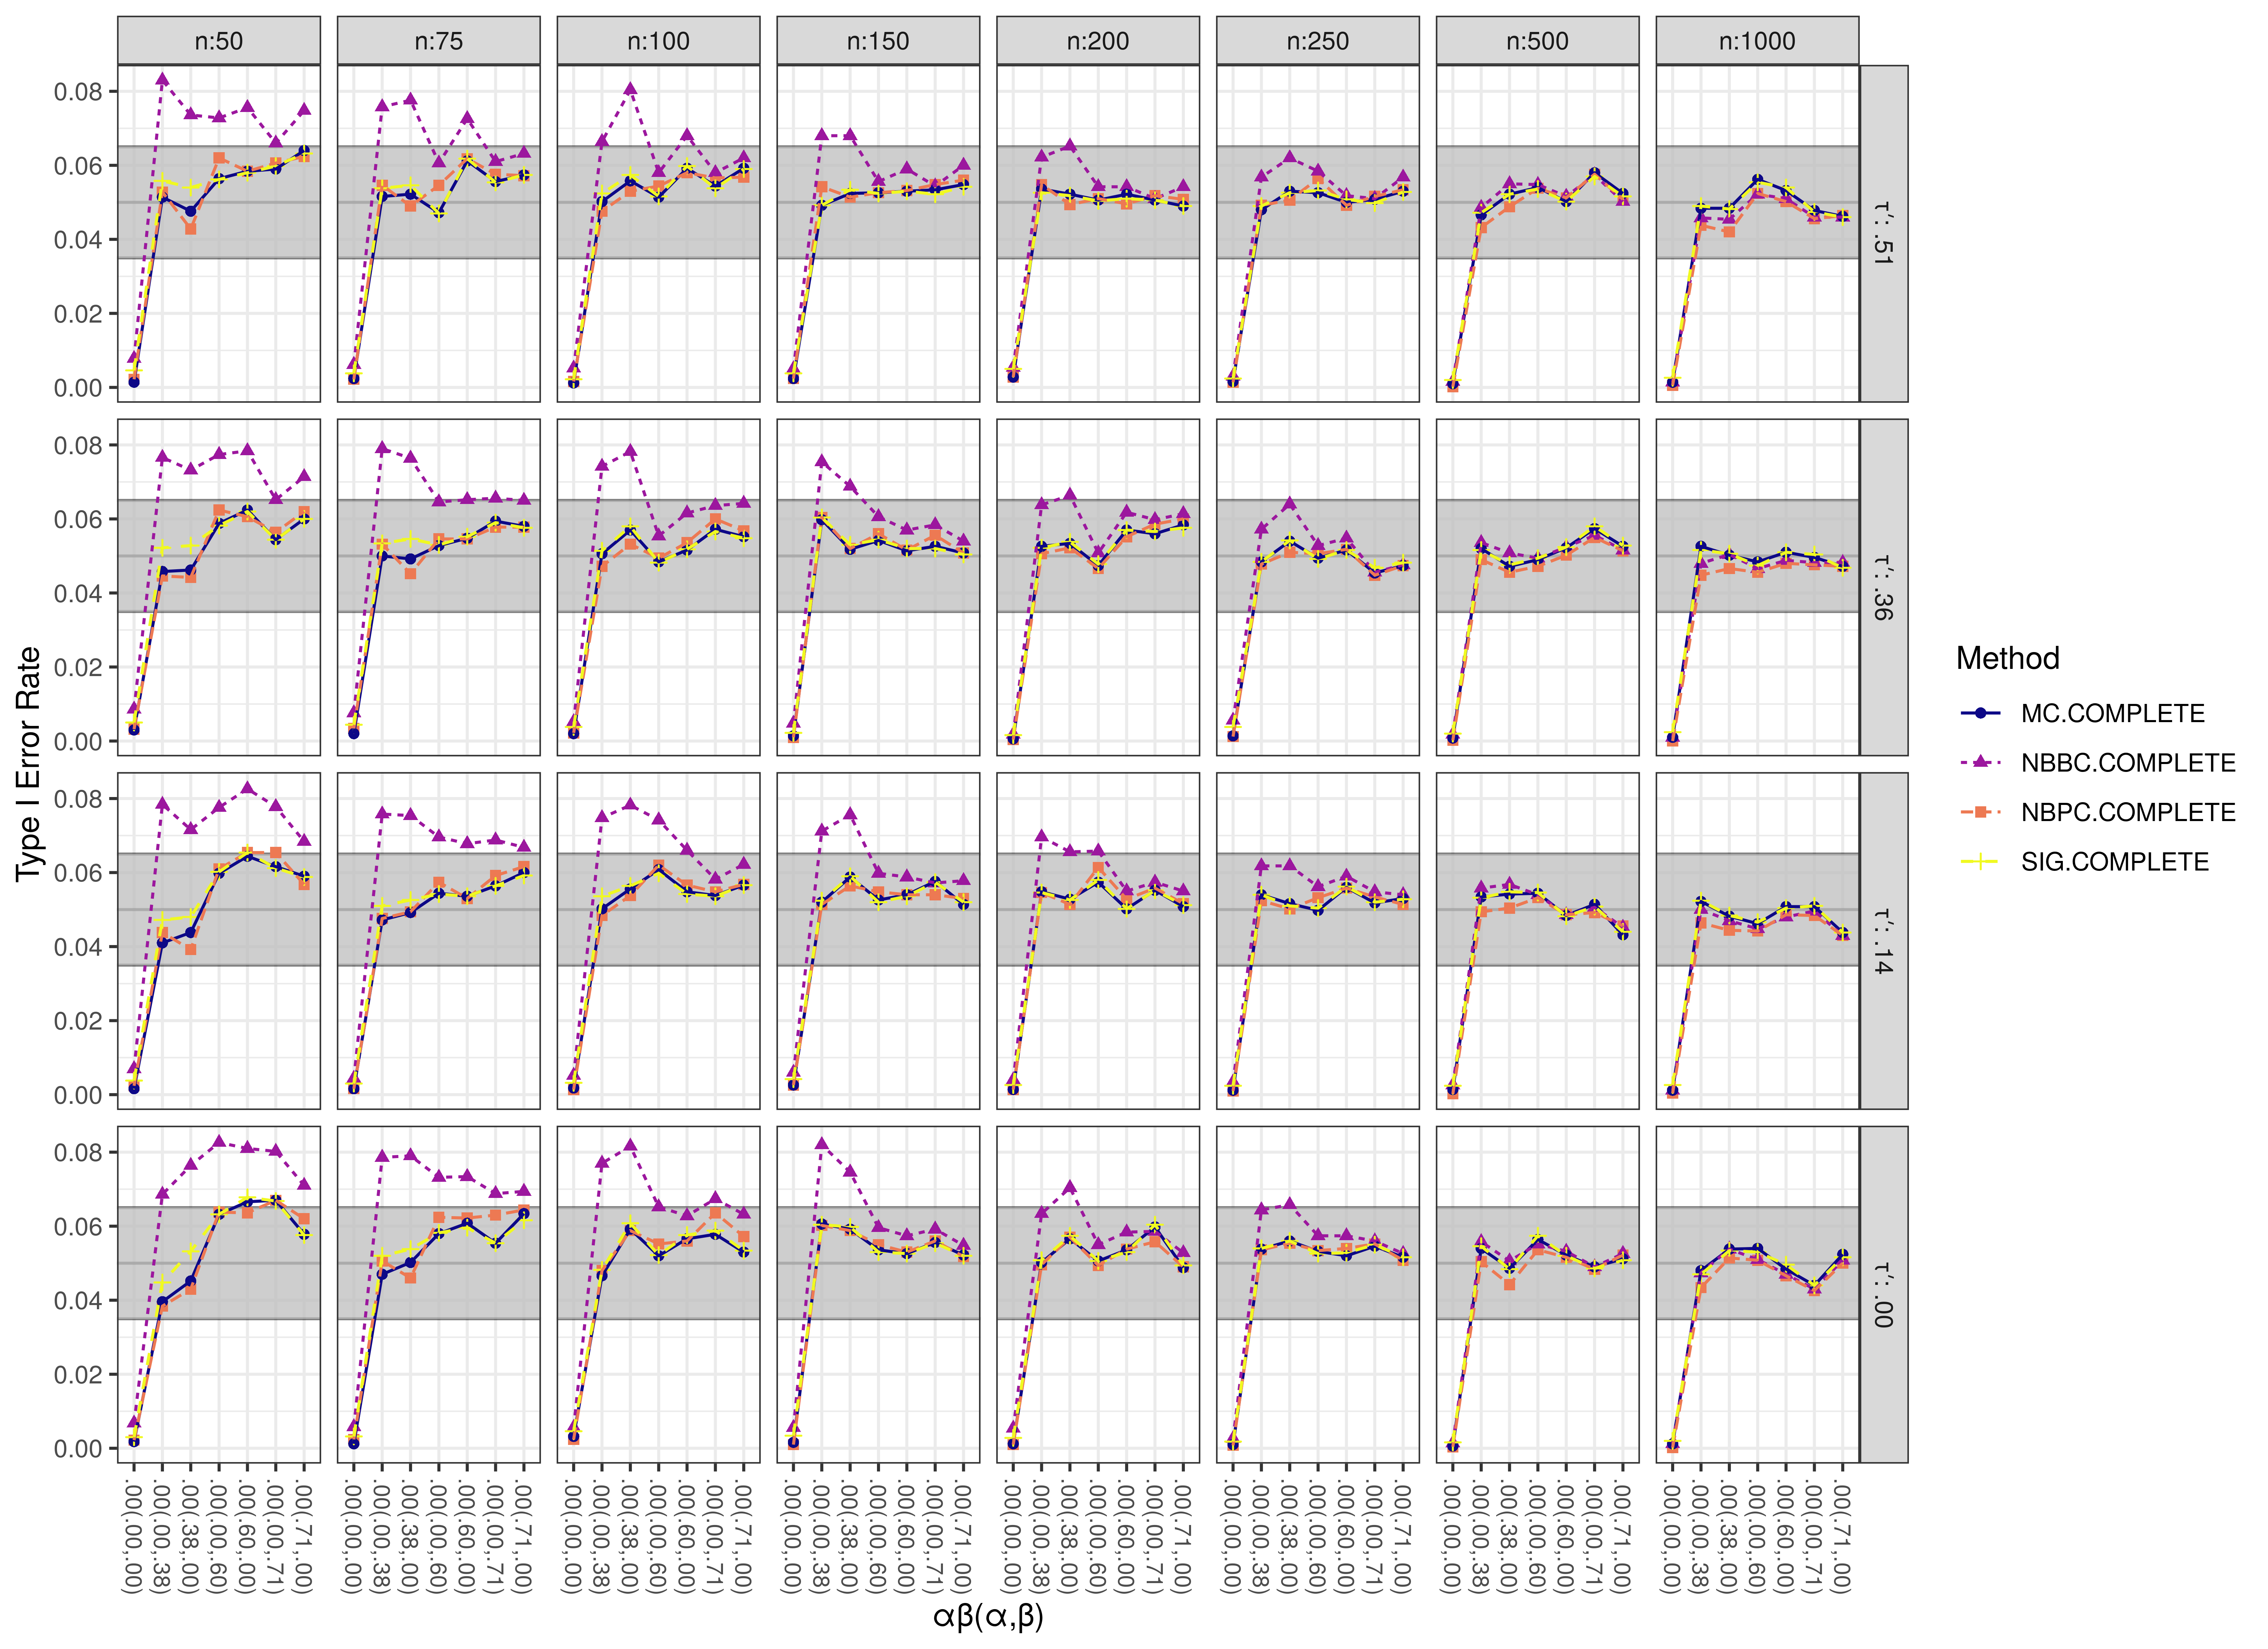
\includegraphics[scale=.60]{figures/png/complete-type1.png}
	\figurenote{
		${n}$ = sample size,
		${\alpha}$ = path from ${X}$ to ${M}$,
		${\beta}$ = path from ${M}$ to ${Y}$,
		${\tau}^{\prime}$ = direct effect,
		MC.COMPLETE = Monte Carlo with complete data,
		NBBC.COMPLETE = Nonparametric bootstrap with bias-corrected confidence intervals with complete data,
        NBPC.COMPLETE = Nonparametric bootstrap with percentile confidence intervals with complete data,
		SIG.COMPLETE = Joint-significance test with complete data.
	}
	\label{fig:complete-type1}
\end{figure}

\newpage

\begin{figure}[ht]
	\caption{
		Type I Error for MCAR (30\% Missing)
	}
	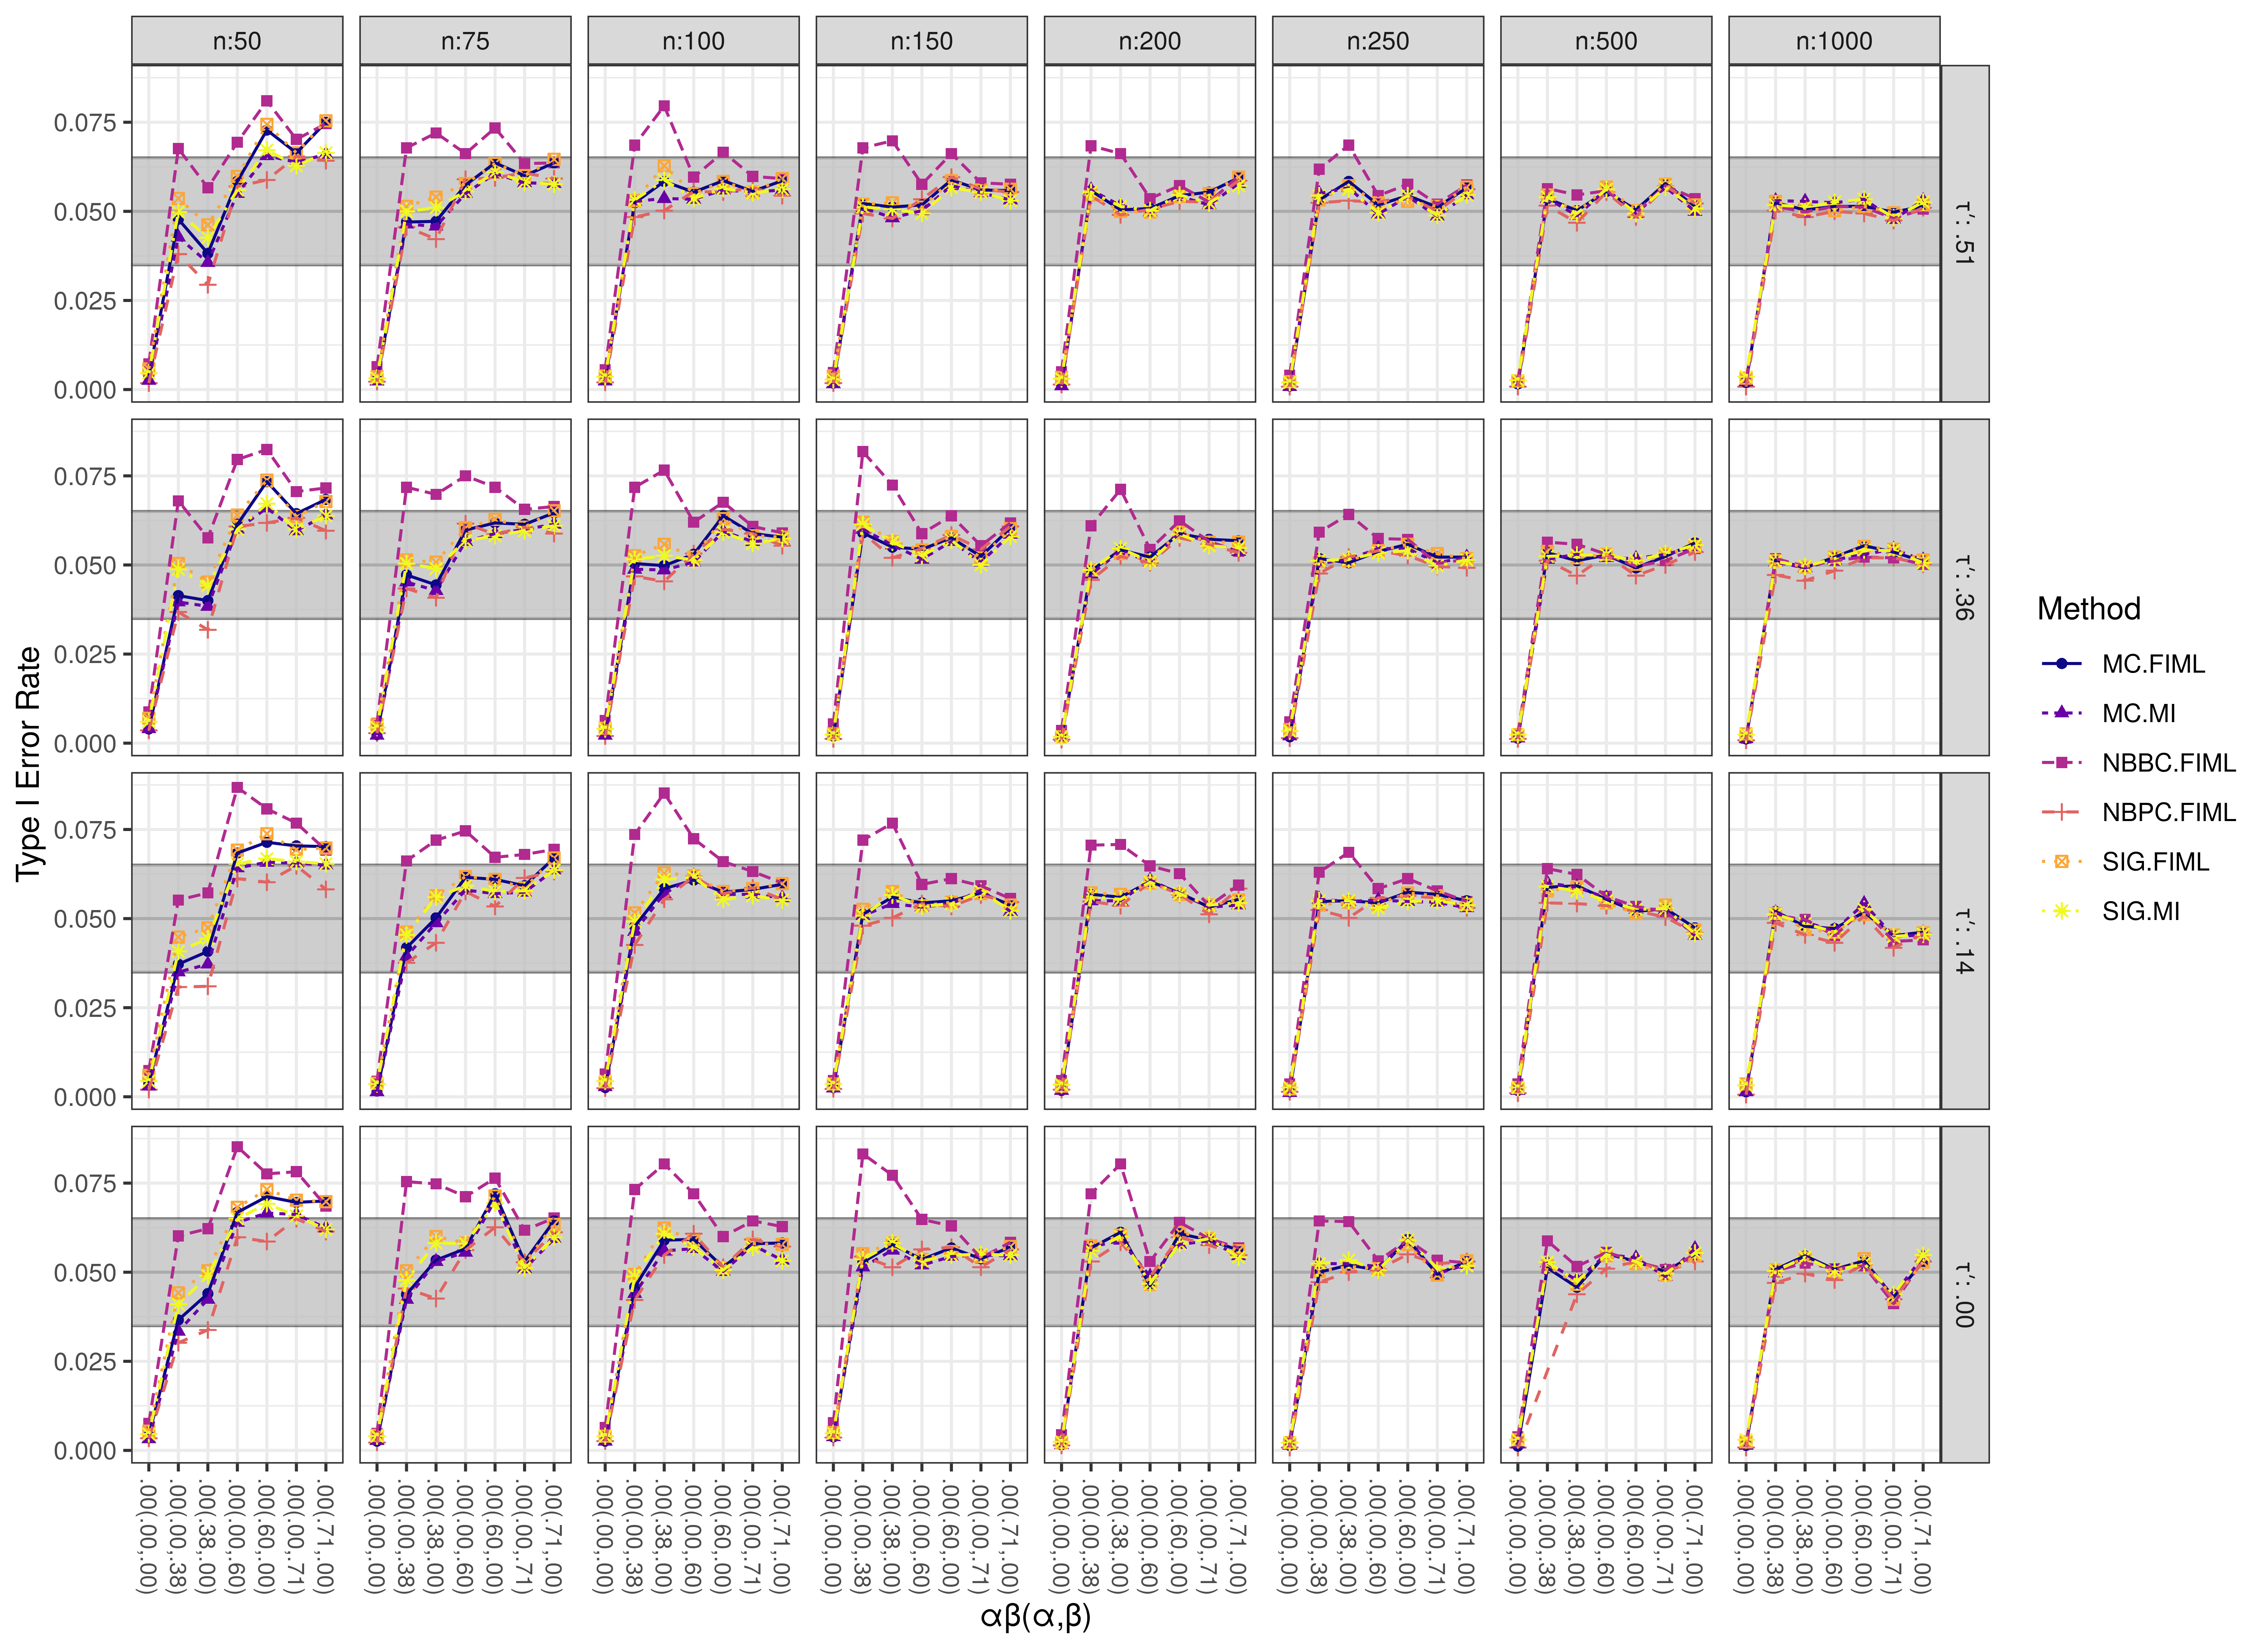
\includegraphics[scale=.60]{figures/png/mcar-30-type1.png}
	\figurenote{
		${n}$ = sample size,
		${\alpha}$ = path from ${X}$ to ${M}$,
		${\beta}$ = path from ${M}$ to ${Y}$,
		${\tau}^{\prime}$ = direct effect,
		MC.FIML = Monte Carlo using FIML estimates,
		MC.MI = Monte Carlo using MI estimates,
		NBBC.FIML = Nonparametric bootstrap with bias-corrected confidence intervals using FIML,
        NBPC.FIML = Nonparametric bootstrap with percentile confidence intervals using FIML,
		SIG.FIML = Joint-significance test using FIML estimates,
		SIG.MI = Joint-significance test using MI estimates.
    }
	\label{fig:mcar-30-type1}
\end{figure}

\newpage

\begin{figure}[ht]
	\caption{
		Type I Error for MAR (30\% Missing)
	}
	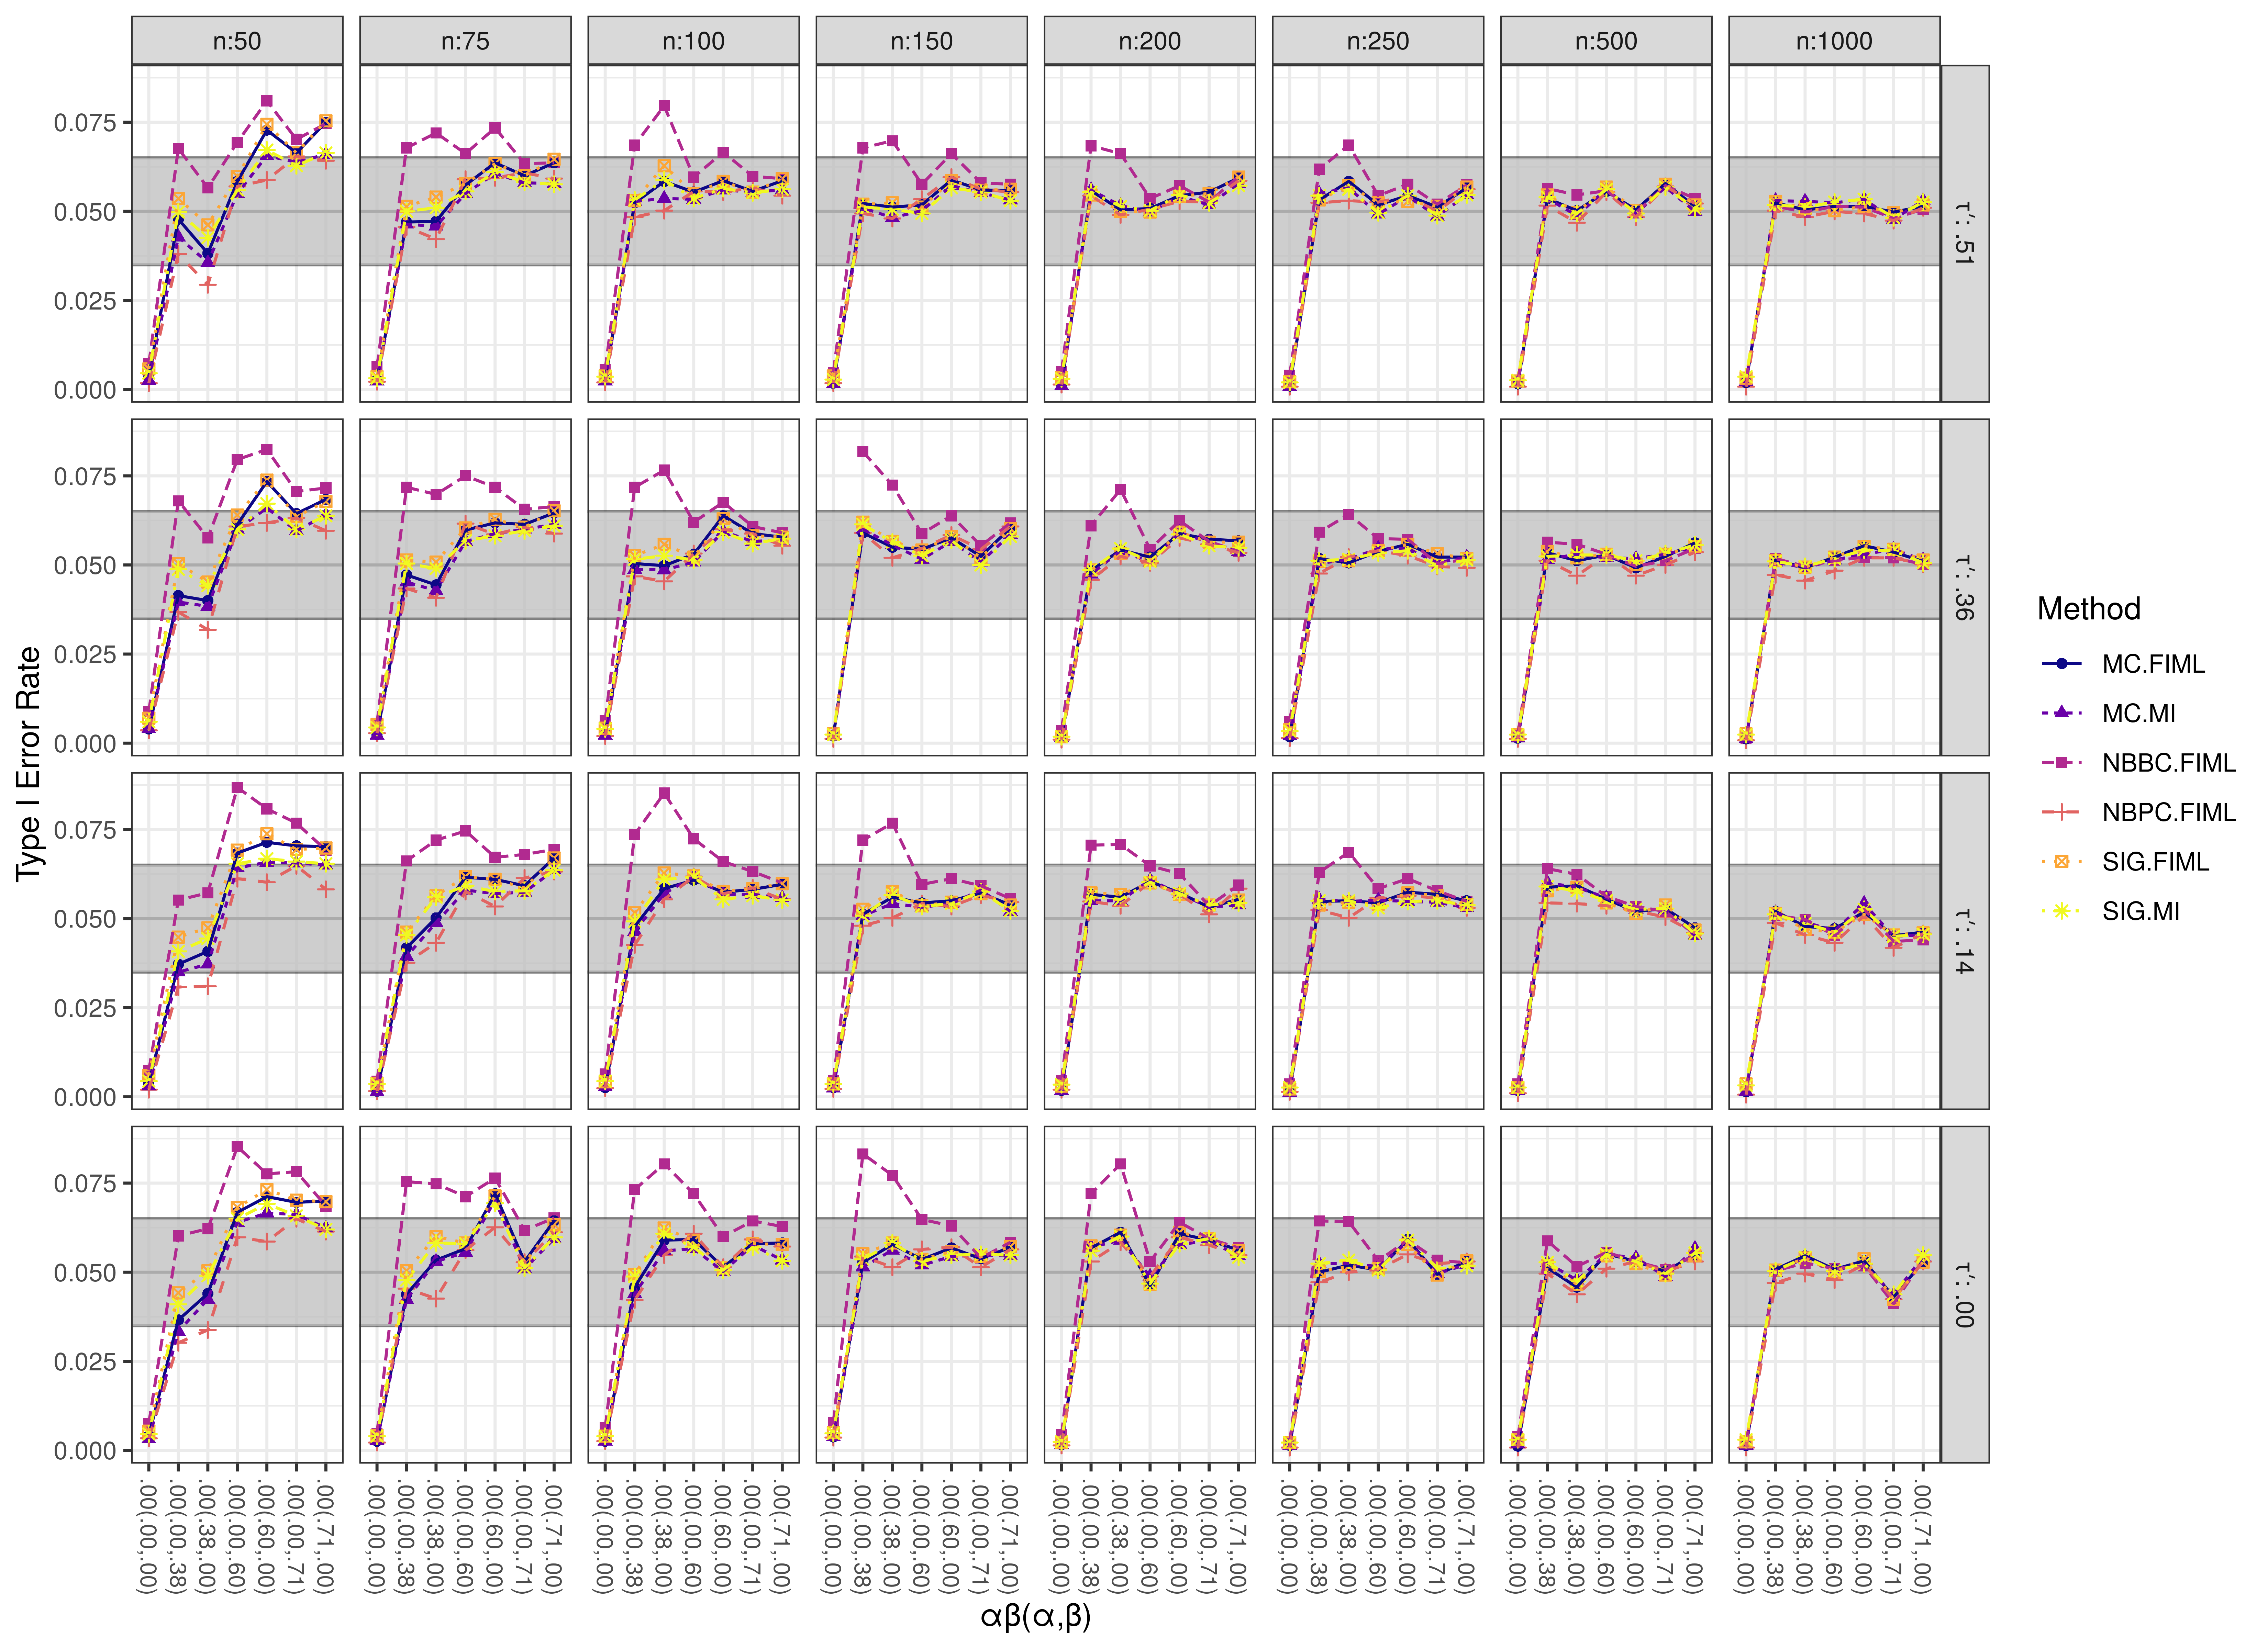
\includegraphics[scale=.60]{figures/png/mar-30-type1.png}
	\figurenote{
		${n}$ = sample size,
		${\alpha}$ = path from ${X}$ to ${M}$,
		${\beta}$ = path from ${M}$ to ${Y}$,
		${\tau}^{\prime}$ = direct effect,
		MC.FIML = Monte Carlo using FIML estimates,
		MC.MI = Monte Carlo using MI estimates,
		NBBC.FIML = Nonparametric bootstrap with bias-corrected confidence intervals using FIML,
        NBPC.FIML = Nonparametric bootstrap with percentile confidence intervals using FIML,
		SIG.FIML = Joint-significance test using FIML estimates,
		SIG.MI = Joint-significance test using MI estimates.
    }
	\label{fig:mar-30-type1}
\end{figure}

% Statistical Power

\begin{figure}[ht]
	\caption{
		Statistical Power for Complete Data
	}
	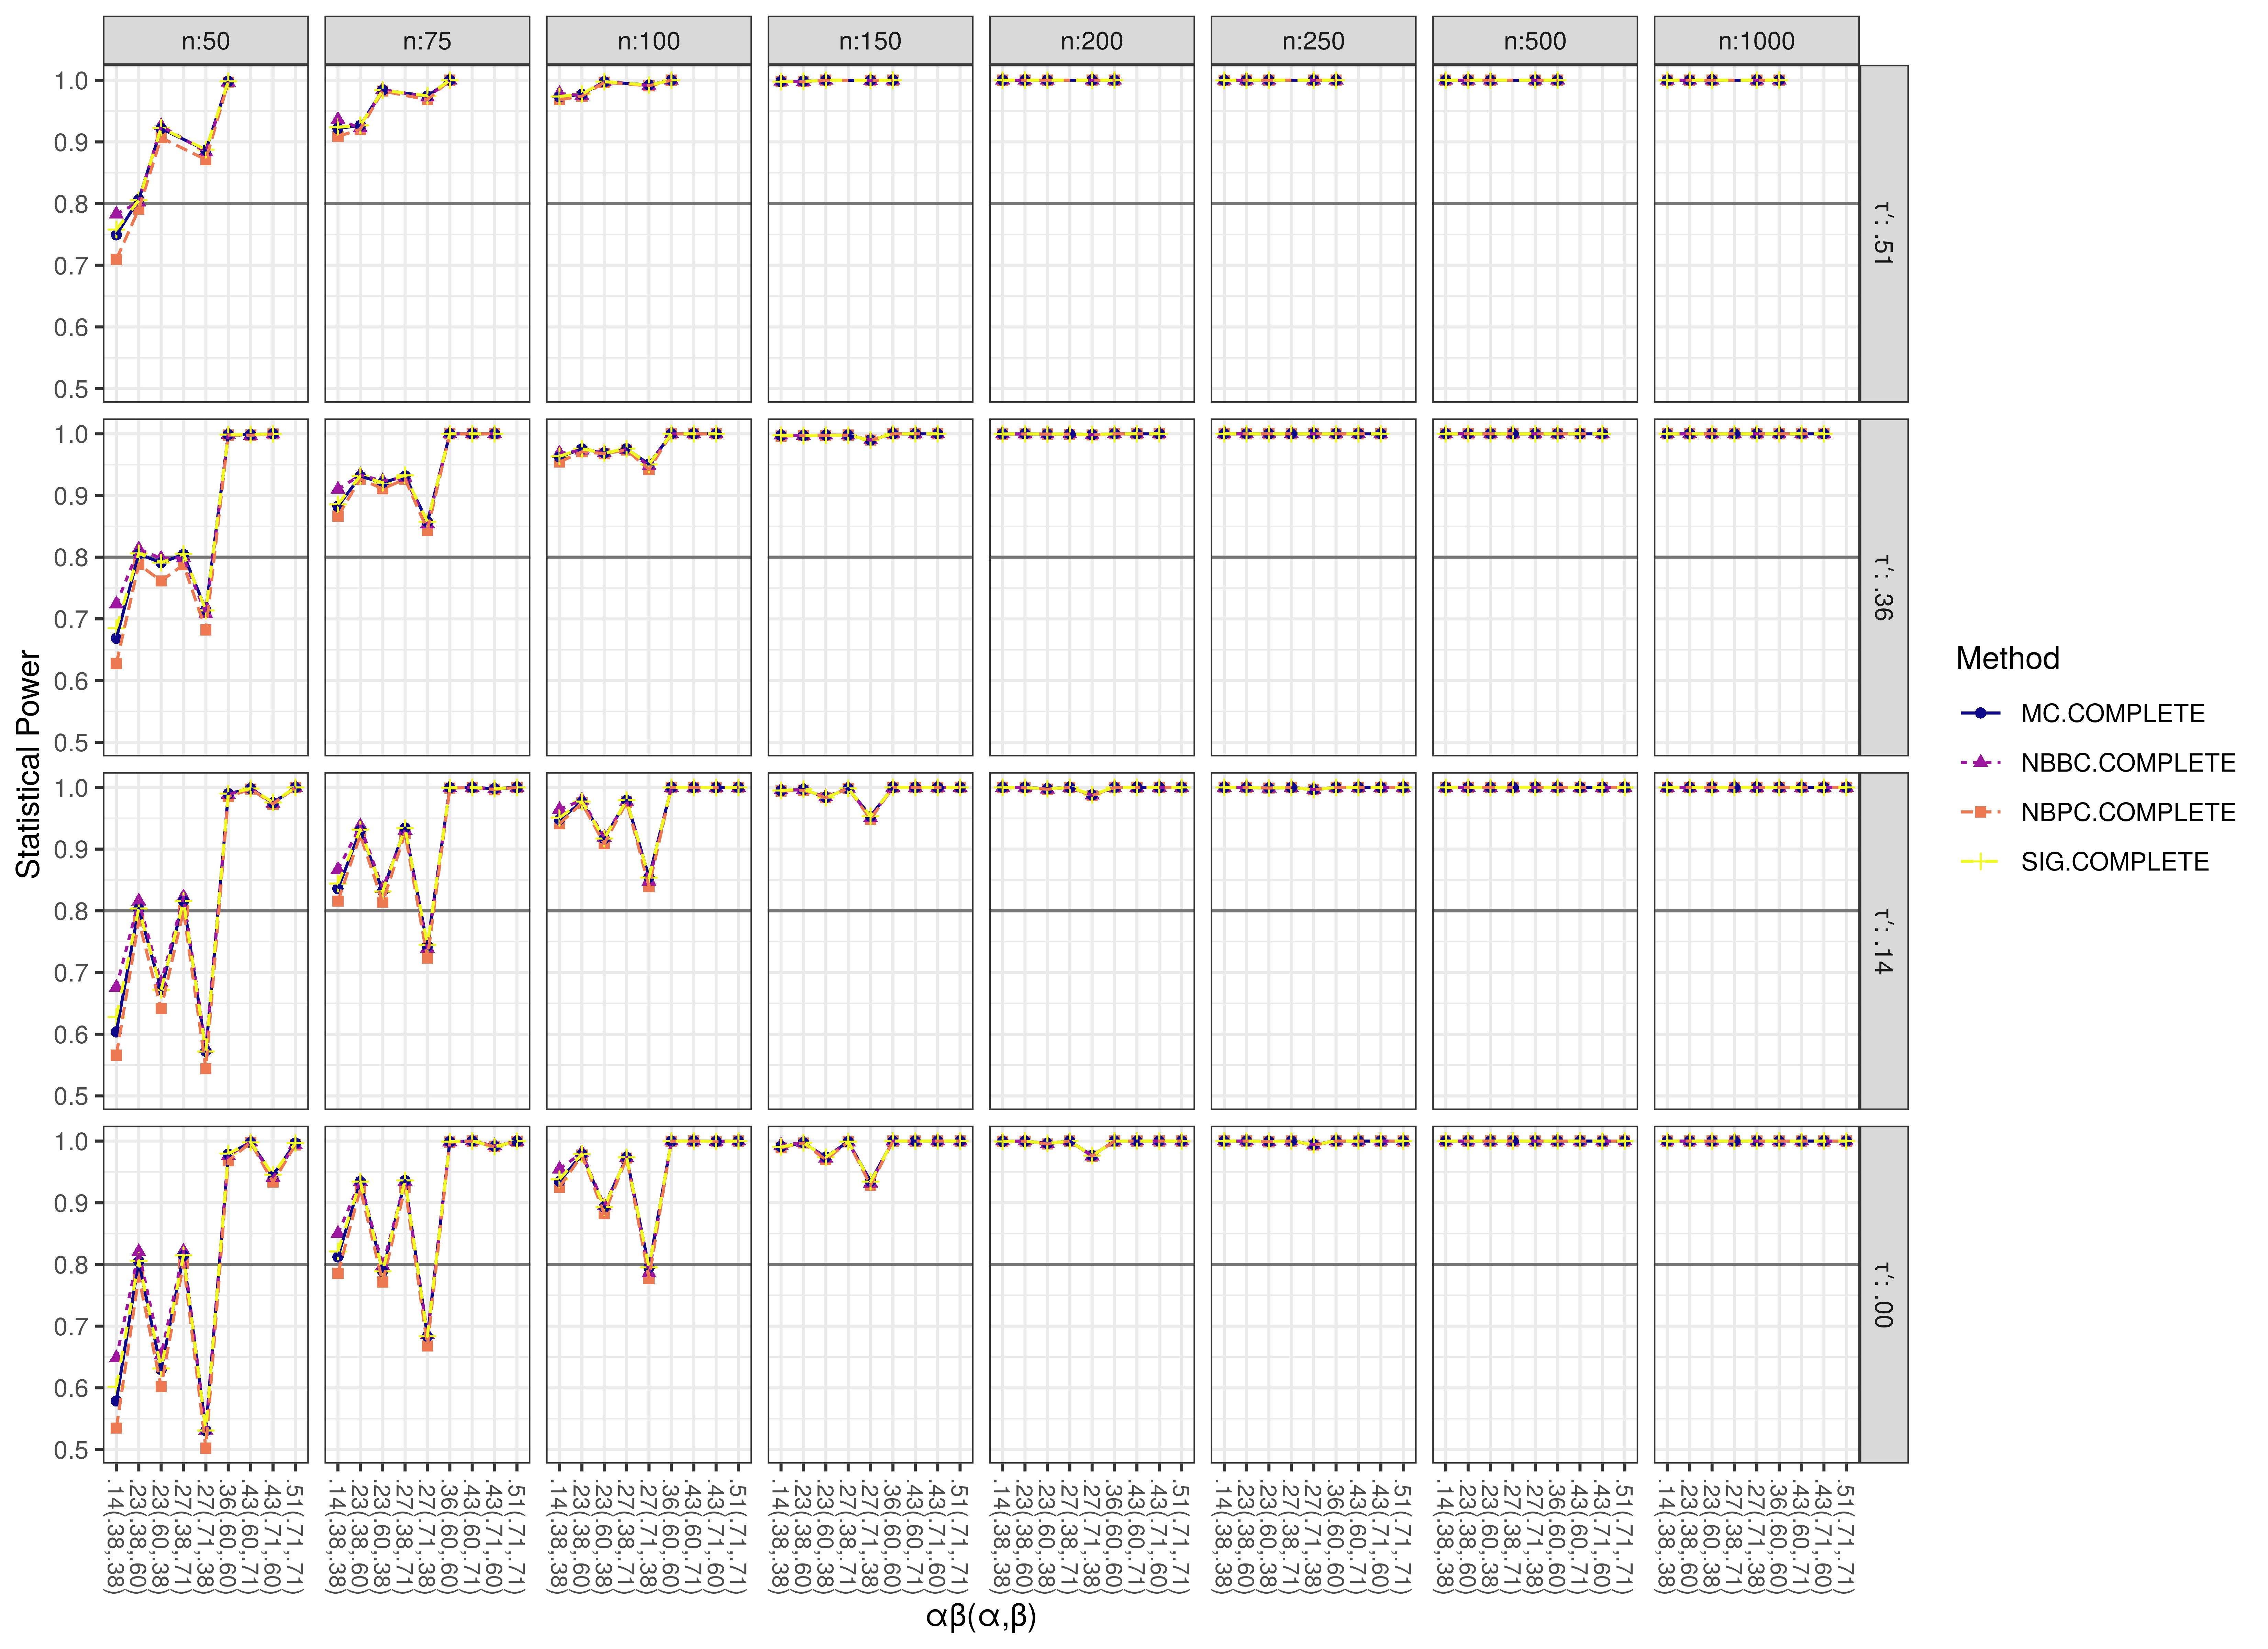
\includegraphics[scale=.60]{figures/png/complete-power.png}
	\figurenote{
		${n}$ = sample size,
		${\alpha}$ = path from ${X}$ to ${M}$,
		${\beta}$ = path from ${M}$ to ${Y}$,
		${\tau}^{\prime}$ = direct effect,
		MC.COMPLETE = Monte Carlo with complete data,
		NBBC.COMPLETE = Nonparametric bootstrap with bias-corrected confidence intervals with complete data,
        NBPC.COMPLETE = Nonparametric bootstrap with percentile confidence intervals with complete data,
		SIG.COMPLETE = Joint-significance test with complete data.
	}
	\label{fig:complete-power}
\end{figure}

\newpage

\begin{figure}[ht]
	\caption{
		Statistical Power for MCAR (30\% Missing)
	}
	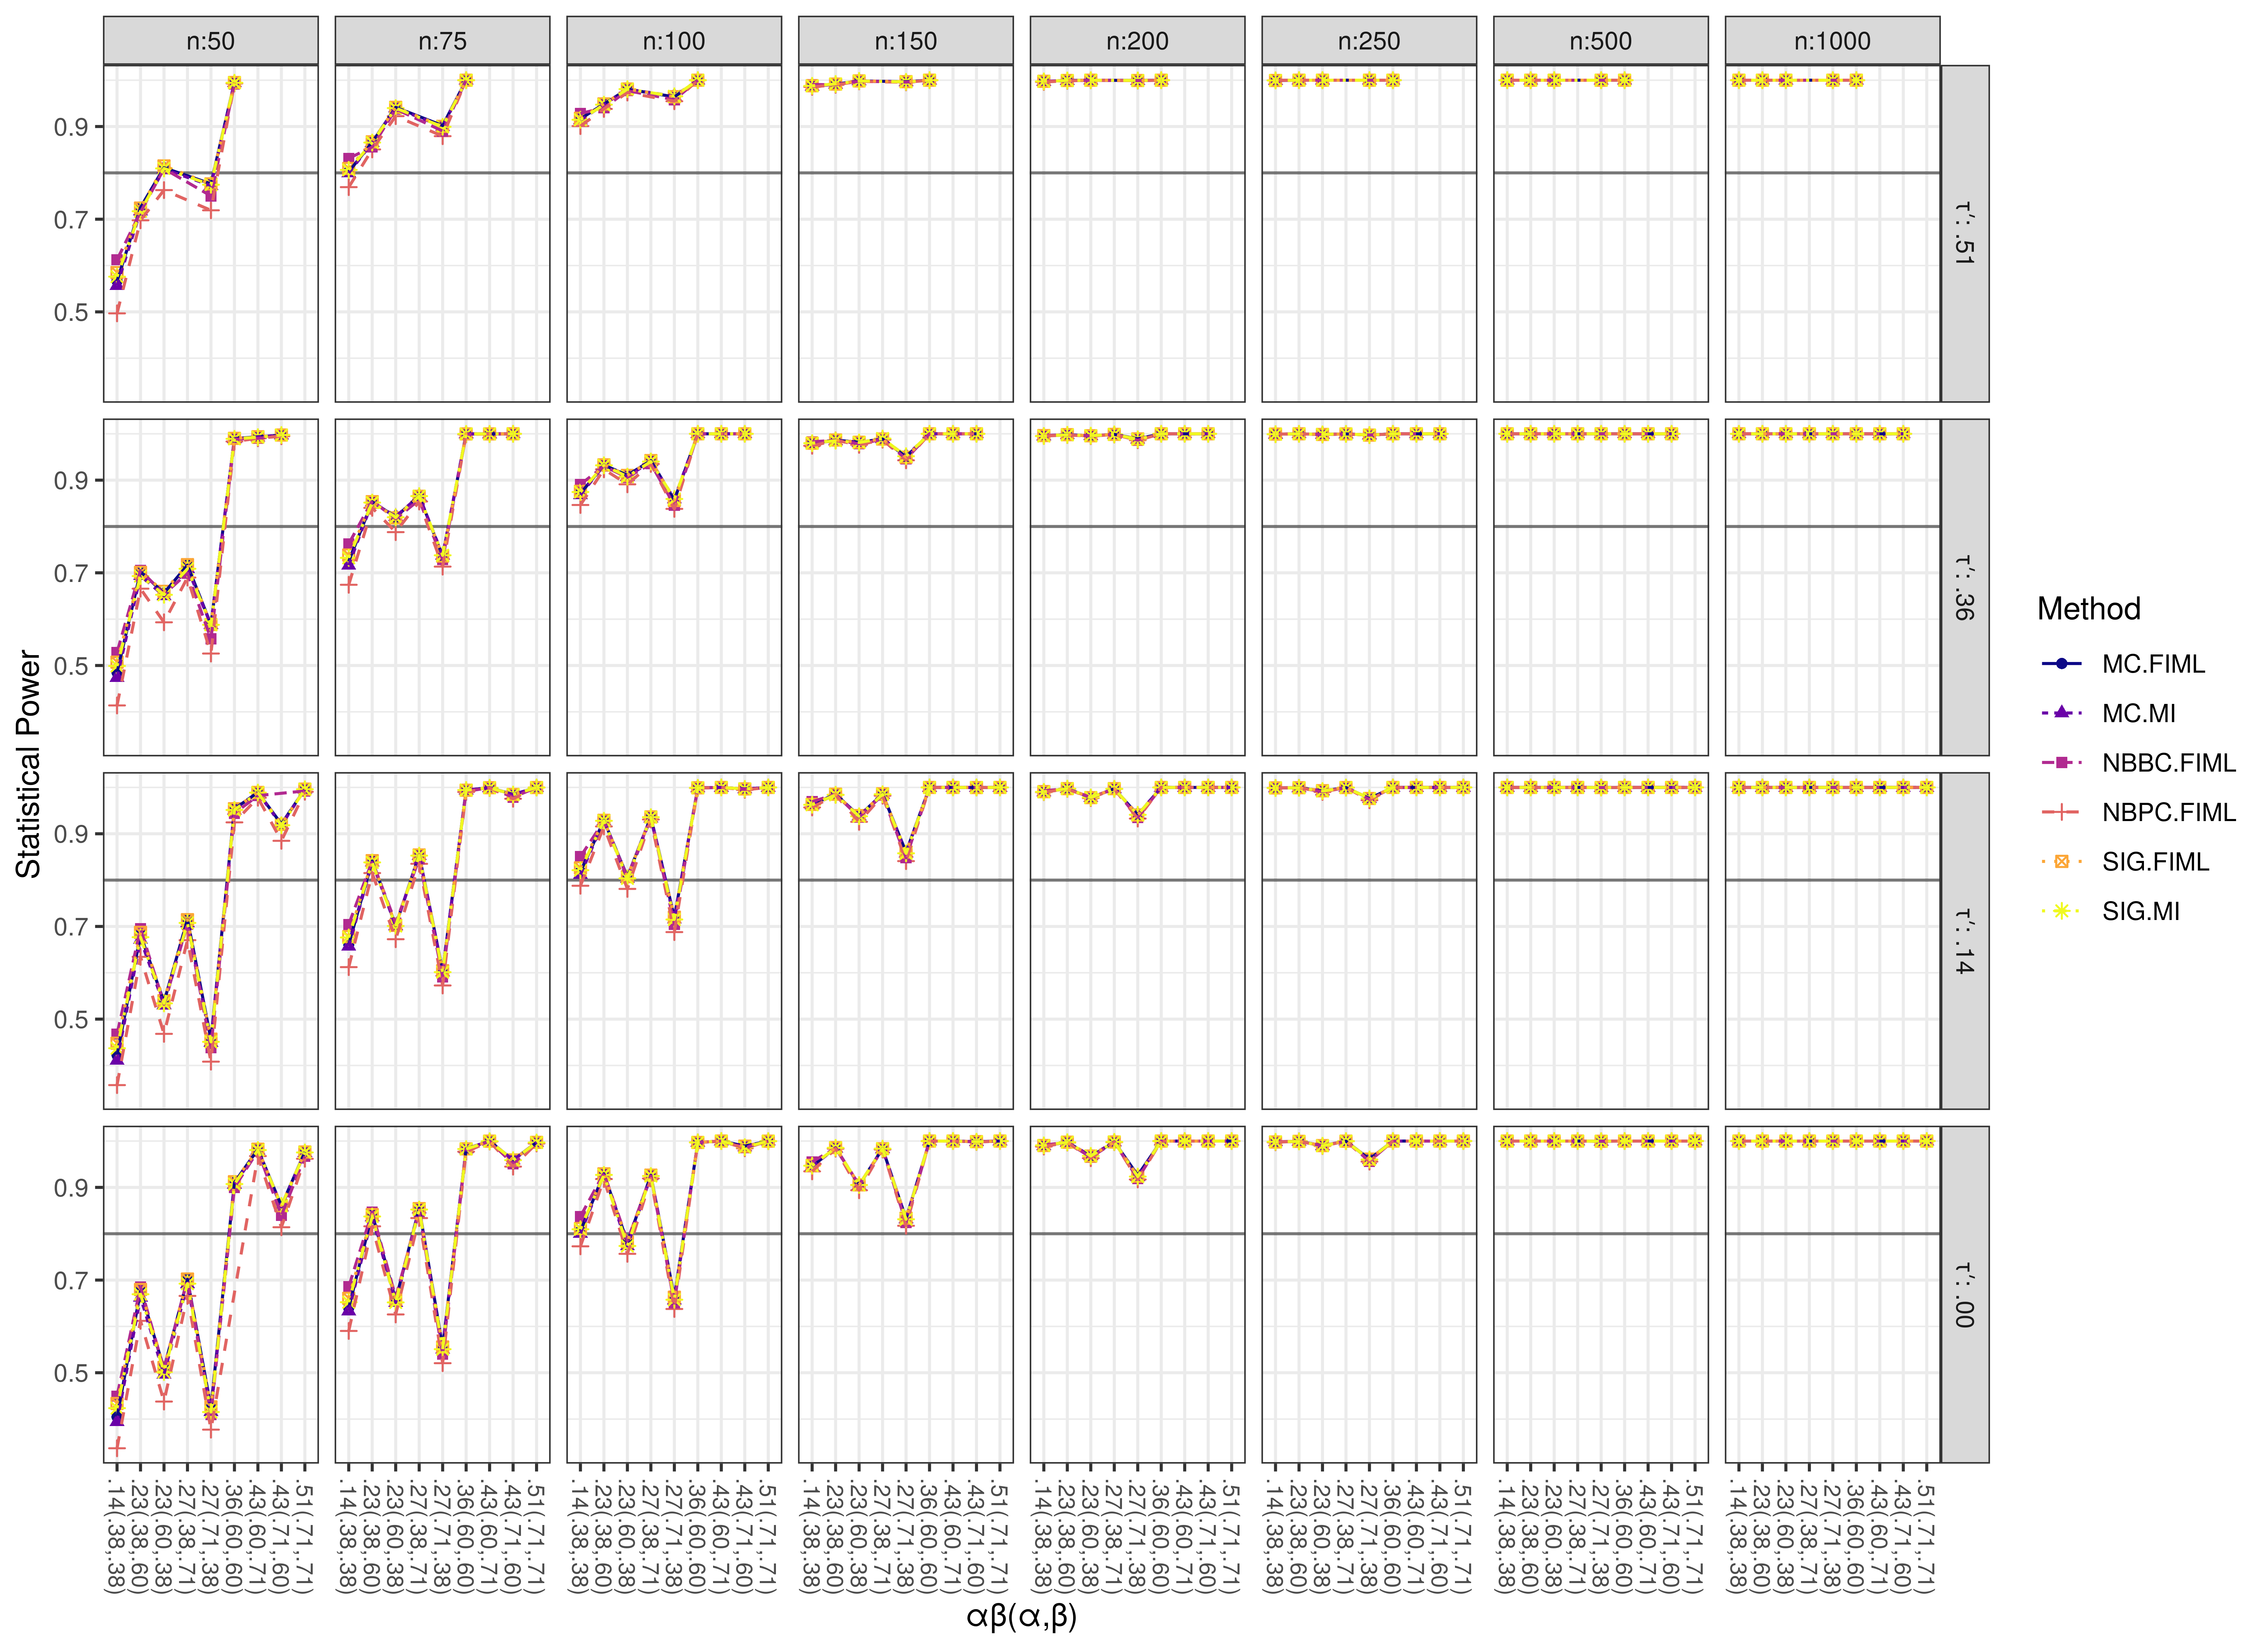
\includegraphics[scale=.60]{figures/png/mcar-30-power.png}
	\figurenote{
		${n}$ = sample size,
		${\alpha}$ = path from ${X}$ to ${M}$,
		${\beta}$ = path from ${M}$ to ${Y}$,
		${\tau}^{\prime}$ = direct effect,
		MC.FIML = Monte Carlo using FIML estimates,
		MC.MI = Monte Carlo using MI estimates,
		NBBC.FIML = Nonparametric bootstrap with bias-corrected confidence intervals using FIML,
        NBPC.FIML = Nonparametric bootstrap with percentile confidence intervals using FIML,
		SIG.FIML = Joint-significance test using FIML estimates,
		SIG.MI = Joint-significance test using MI estimates.
    }
	\label{fig:mcar-30-power}
\end{figure}

\newpage

\begin{figure}[ht]
	\caption{
		Statistical Power for MAR (30\% Missing)
	}
	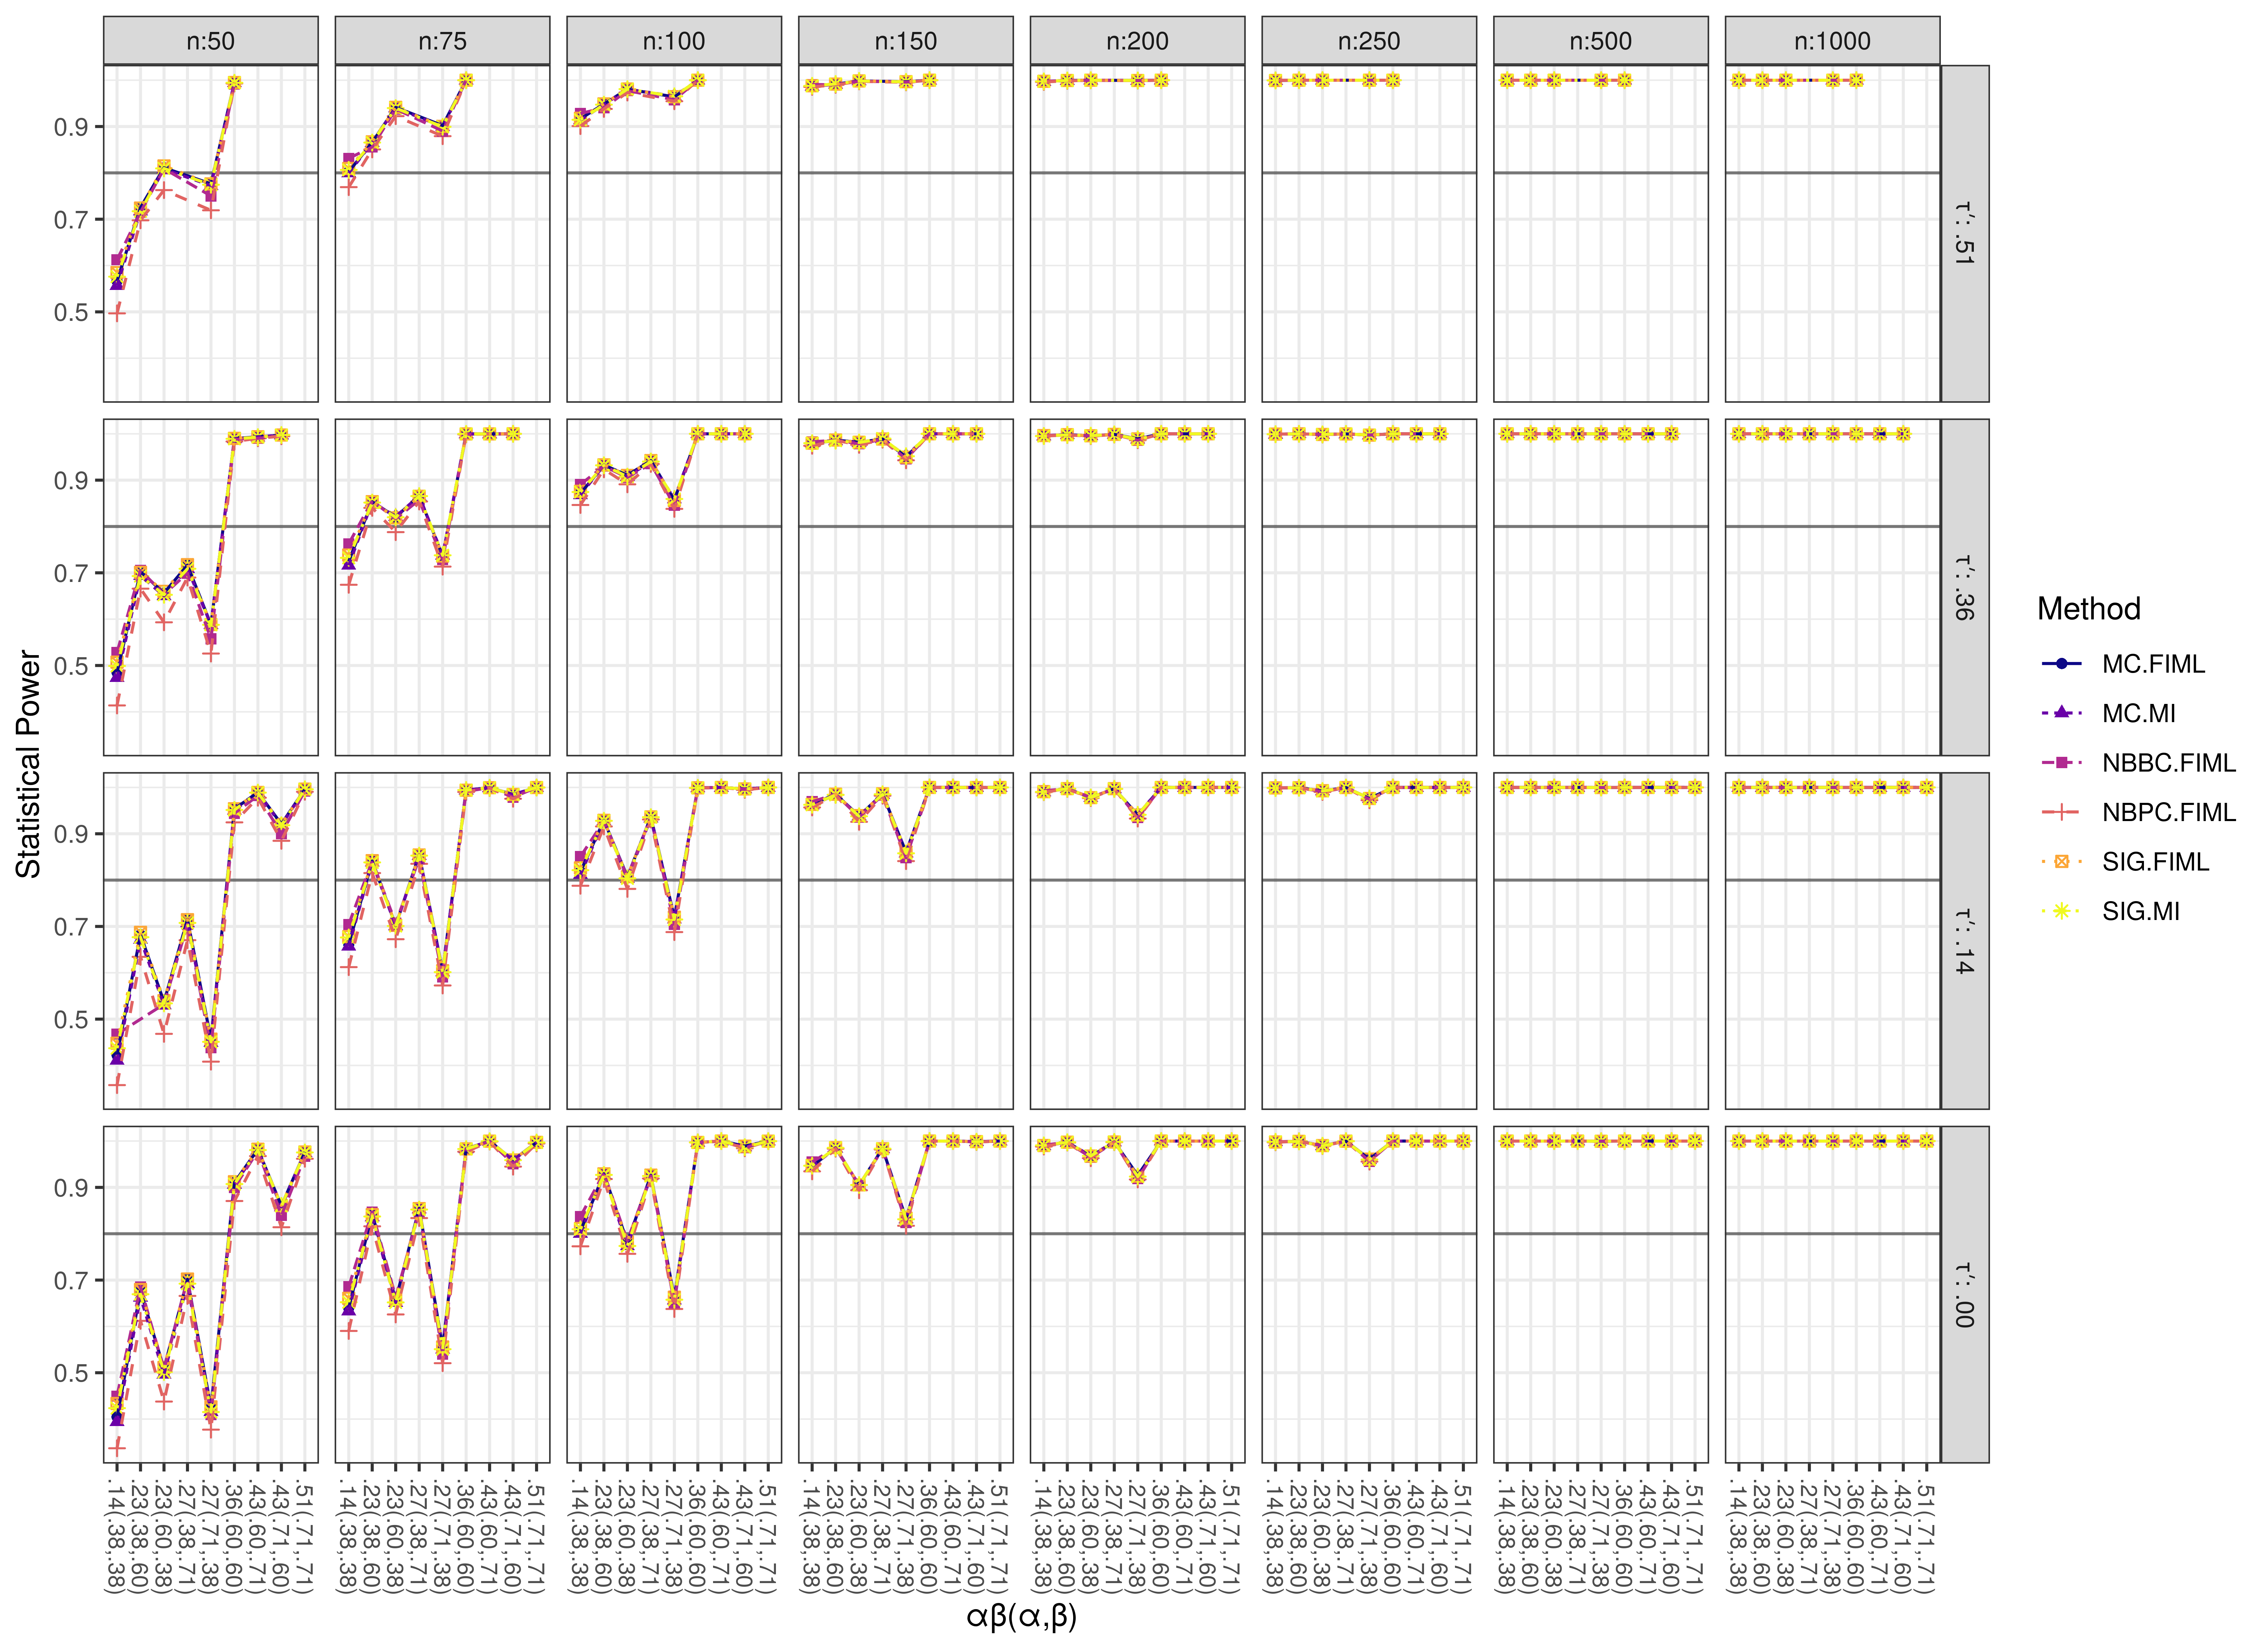
\includegraphics[scale=.60]{figures/png/mar-30-power.png}
	\figurenote{
		${n}$ = sample size,
		${\alpha}$ = path from ${X}$ to ${M}$,
		${\beta}$ = path from ${M}$ to ${Y}$,
		${\tau}^{\prime}$ = direct effect,
		MC.FIML = Monte Carlo using FIML estimates,
		MC.MI = Monte Carlo using MI estimates,
		NBBC.FIML = Nonparametric bootstrap with bias-corrected confidence intervals using FIML,
        NBPC.FIML = Nonparametric bootstrap with percentile confidence intervals using FIML,
		SIG.FIML = Joint-significance test using FIML estimates,
		SIG.MI = Joint-significance test using MI estimates.
    }
	\label{fig:mar-30-power}
\end{figure}

\newpage

% Miss Rate

\begin{figure}[ht]
	\caption{
		Miss Rate for Complete Data
	}
	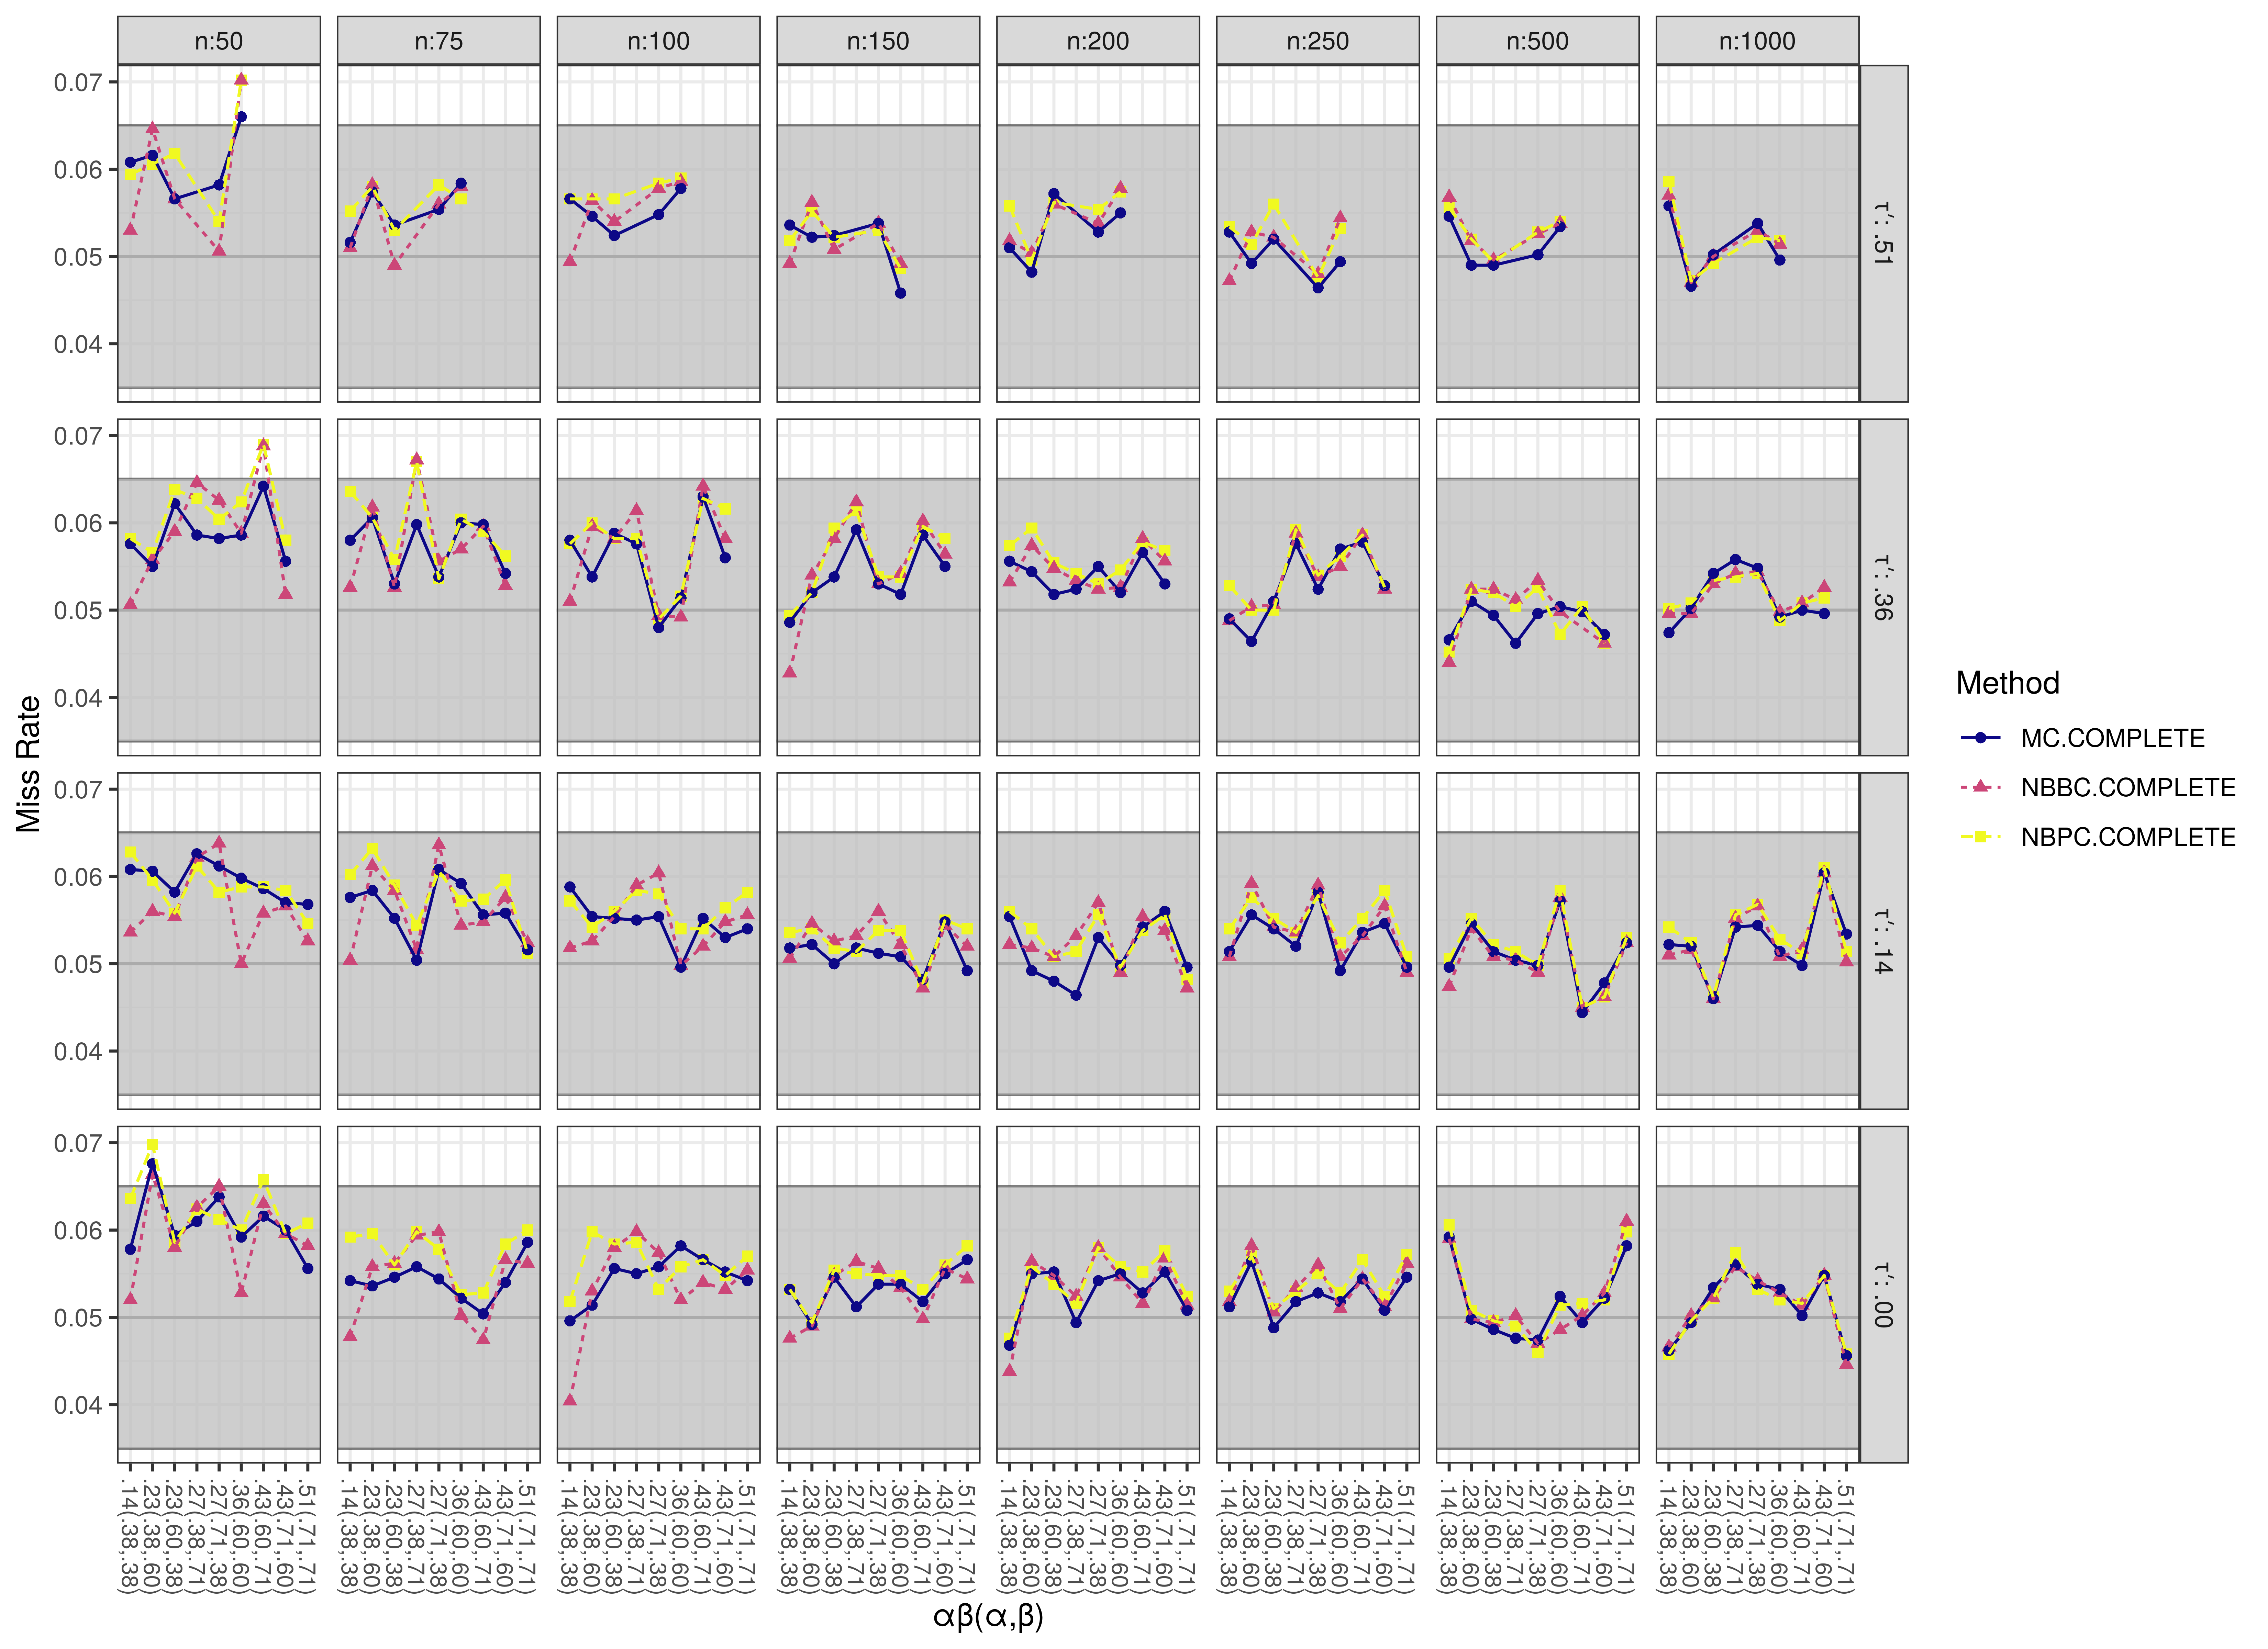
\includegraphics[scale=.60]{figures/png/complete-miss.png}
	\figurenote{
		${n}$ = sample size,
		${\alpha}$ = path from ${X}$ to ${M}$,
		${\beta}$ = path from ${M}$ to ${Y}$,
		${\tau}^{\prime}$ = direct effect,
		MC.COMPLETE = Monte Carlo with complete data,
		NBBC.COMPLETE = Nonparametric bootstrap with bias-corrected confidence intervals with complete data,
        NBPC.COMPLETE = Nonparametric bootstrap with percentile confidence intervals with complete data.
	}
	\label{fig:complete-miss}
\end{figure}

\newpage

\begin{figure}[ht]
	\caption{
		Miss Rate for MCAR (30\% Missing)
	}
	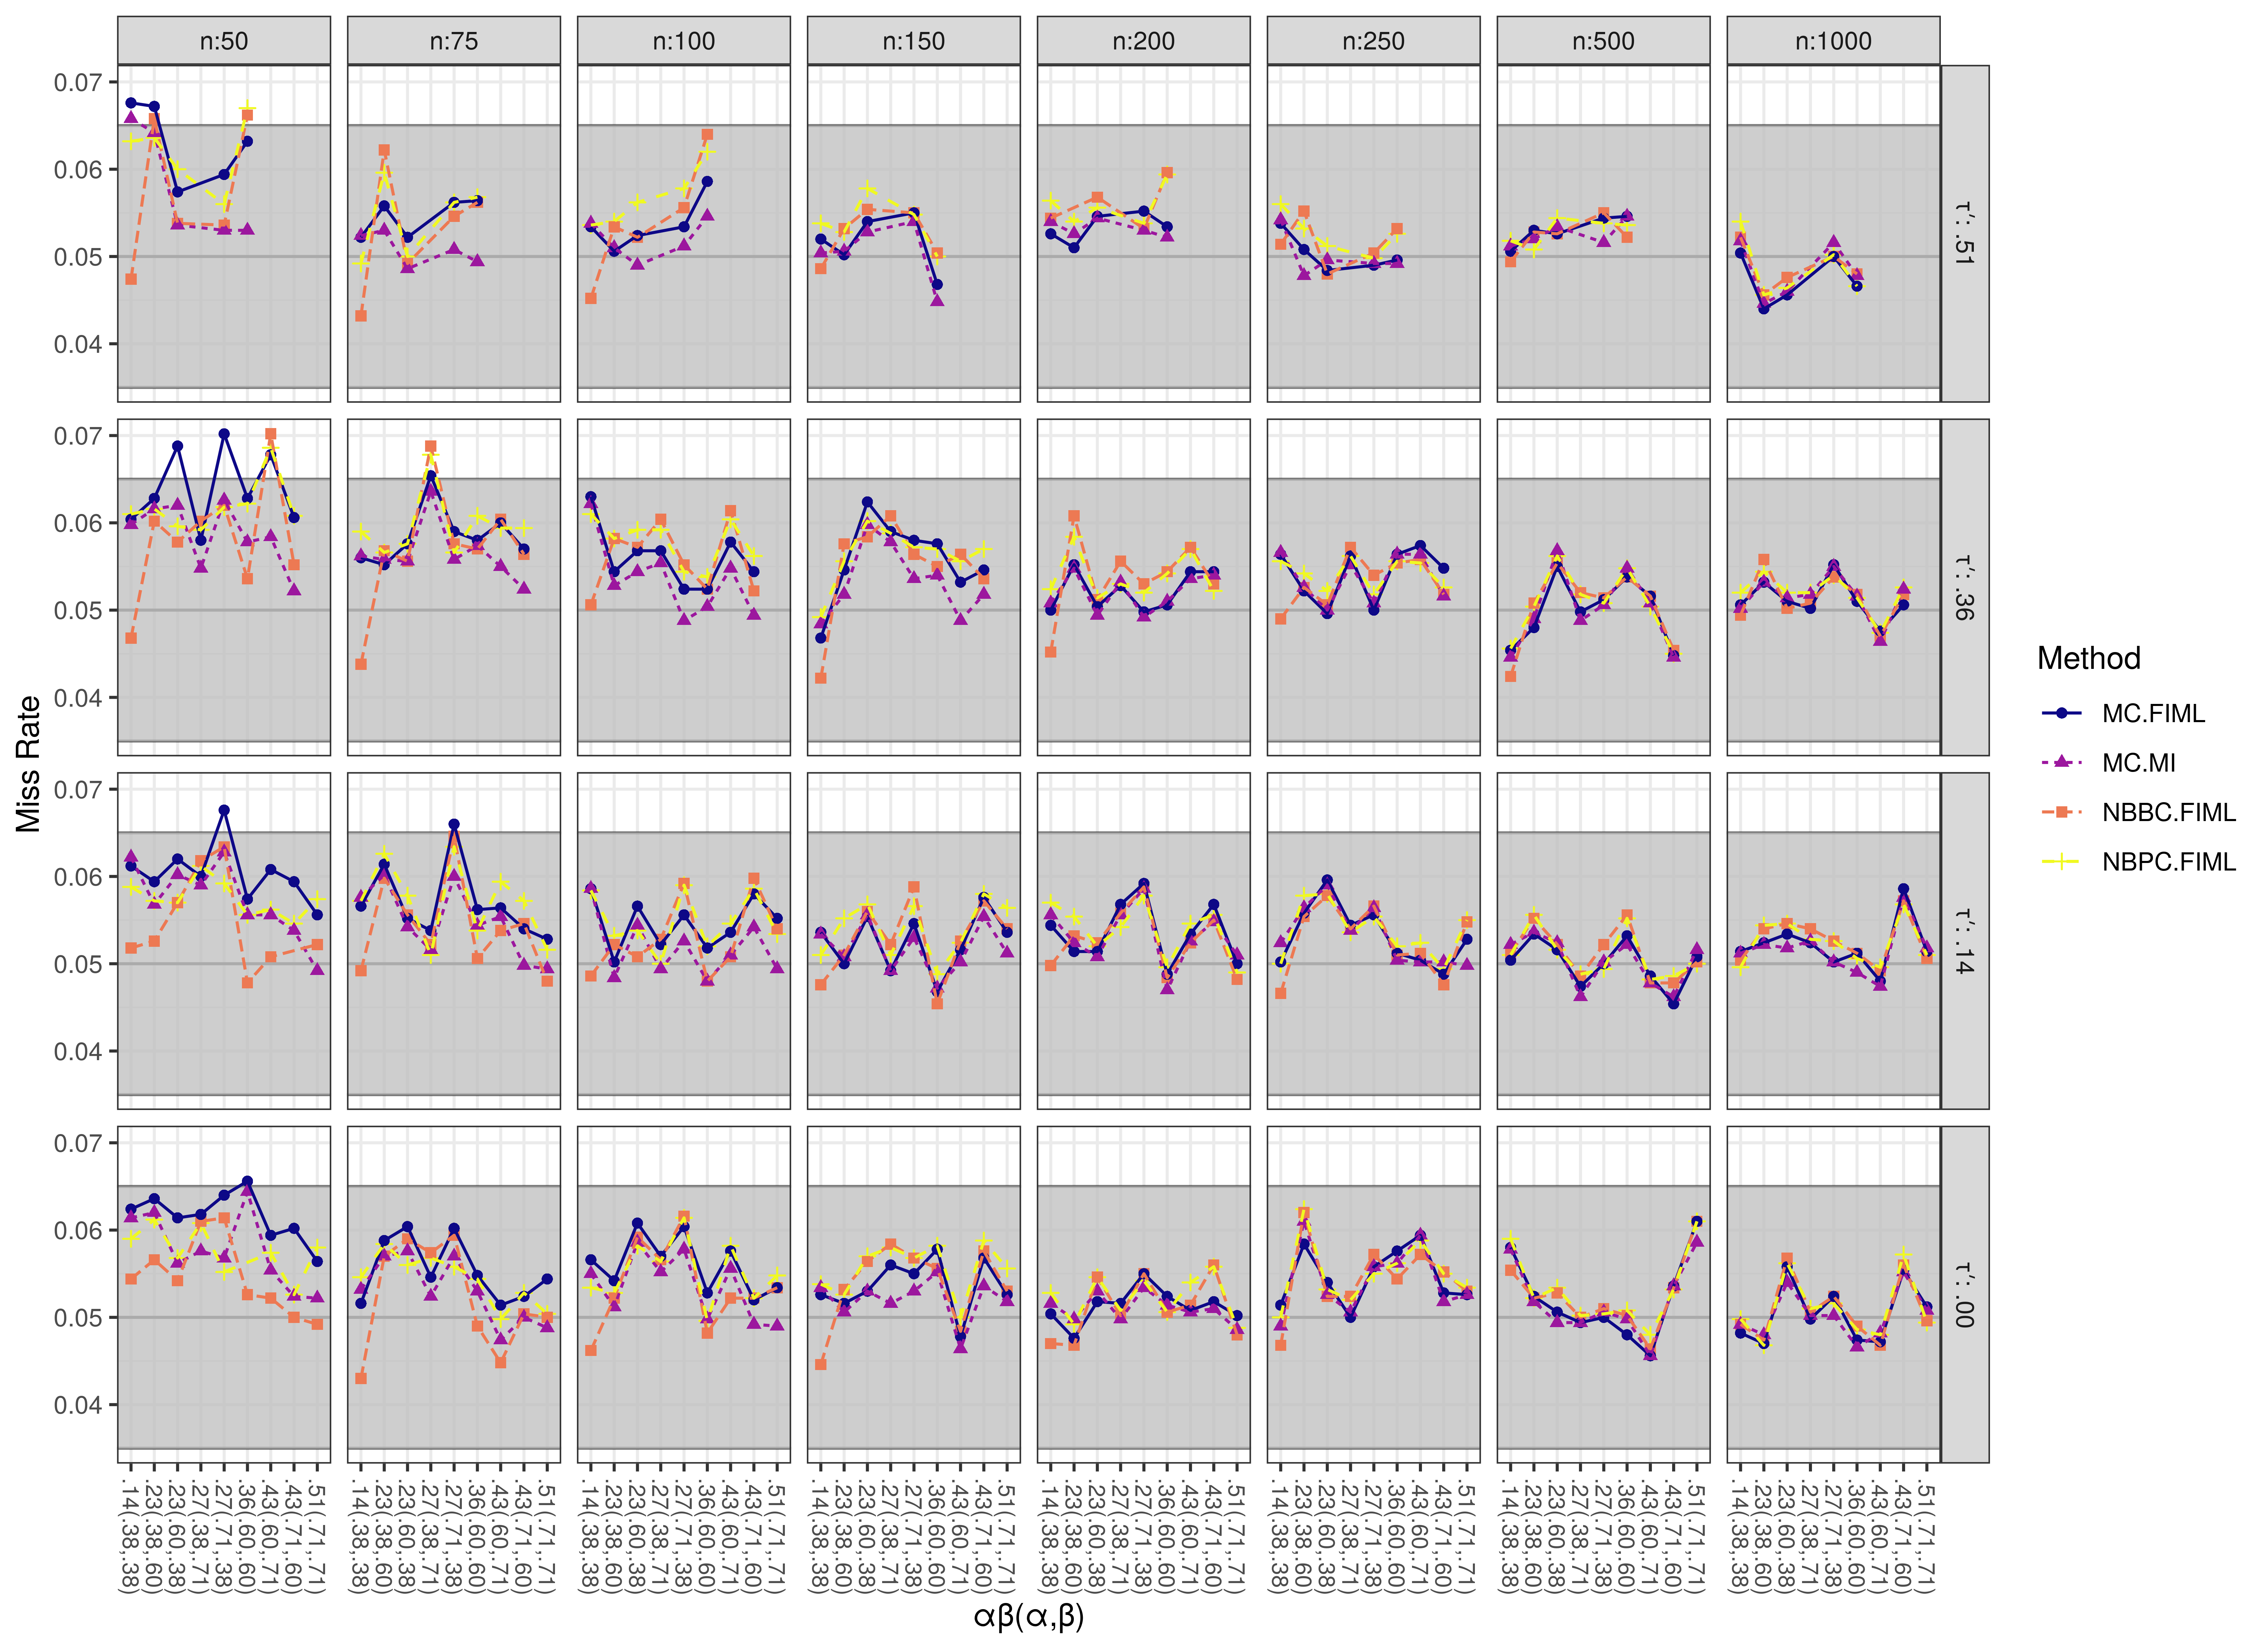
\includegraphics[scale=.60]{figures/png/mcar-30-miss.png}
	\figurenote{
		${n}$ = sample size,
		${\alpha}$ = path from ${X}$ to ${M}$,
		${\beta}$ = path from ${M}$ to ${Y}$,
		${\tau}^{\prime}$ = direct effect,
		MC.FIML = Monte Carlo using FIML estimates,
		MC.MI = Monte Carlo using MI estimates,
		NBBC.FIML = Nonparametric bootstrap with bias-corrected confidence intervals using FIML,
        NBPC.FIML = Nonparametric bootstrap with percentile confidence intervals using FIML.
    }
	\label{fig:mcar-30-miss}
\end{figure}

\newpage

\begin{figure}[ht]
	\caption{
		Miss Rate for MAR (30\% Missing)
	}
	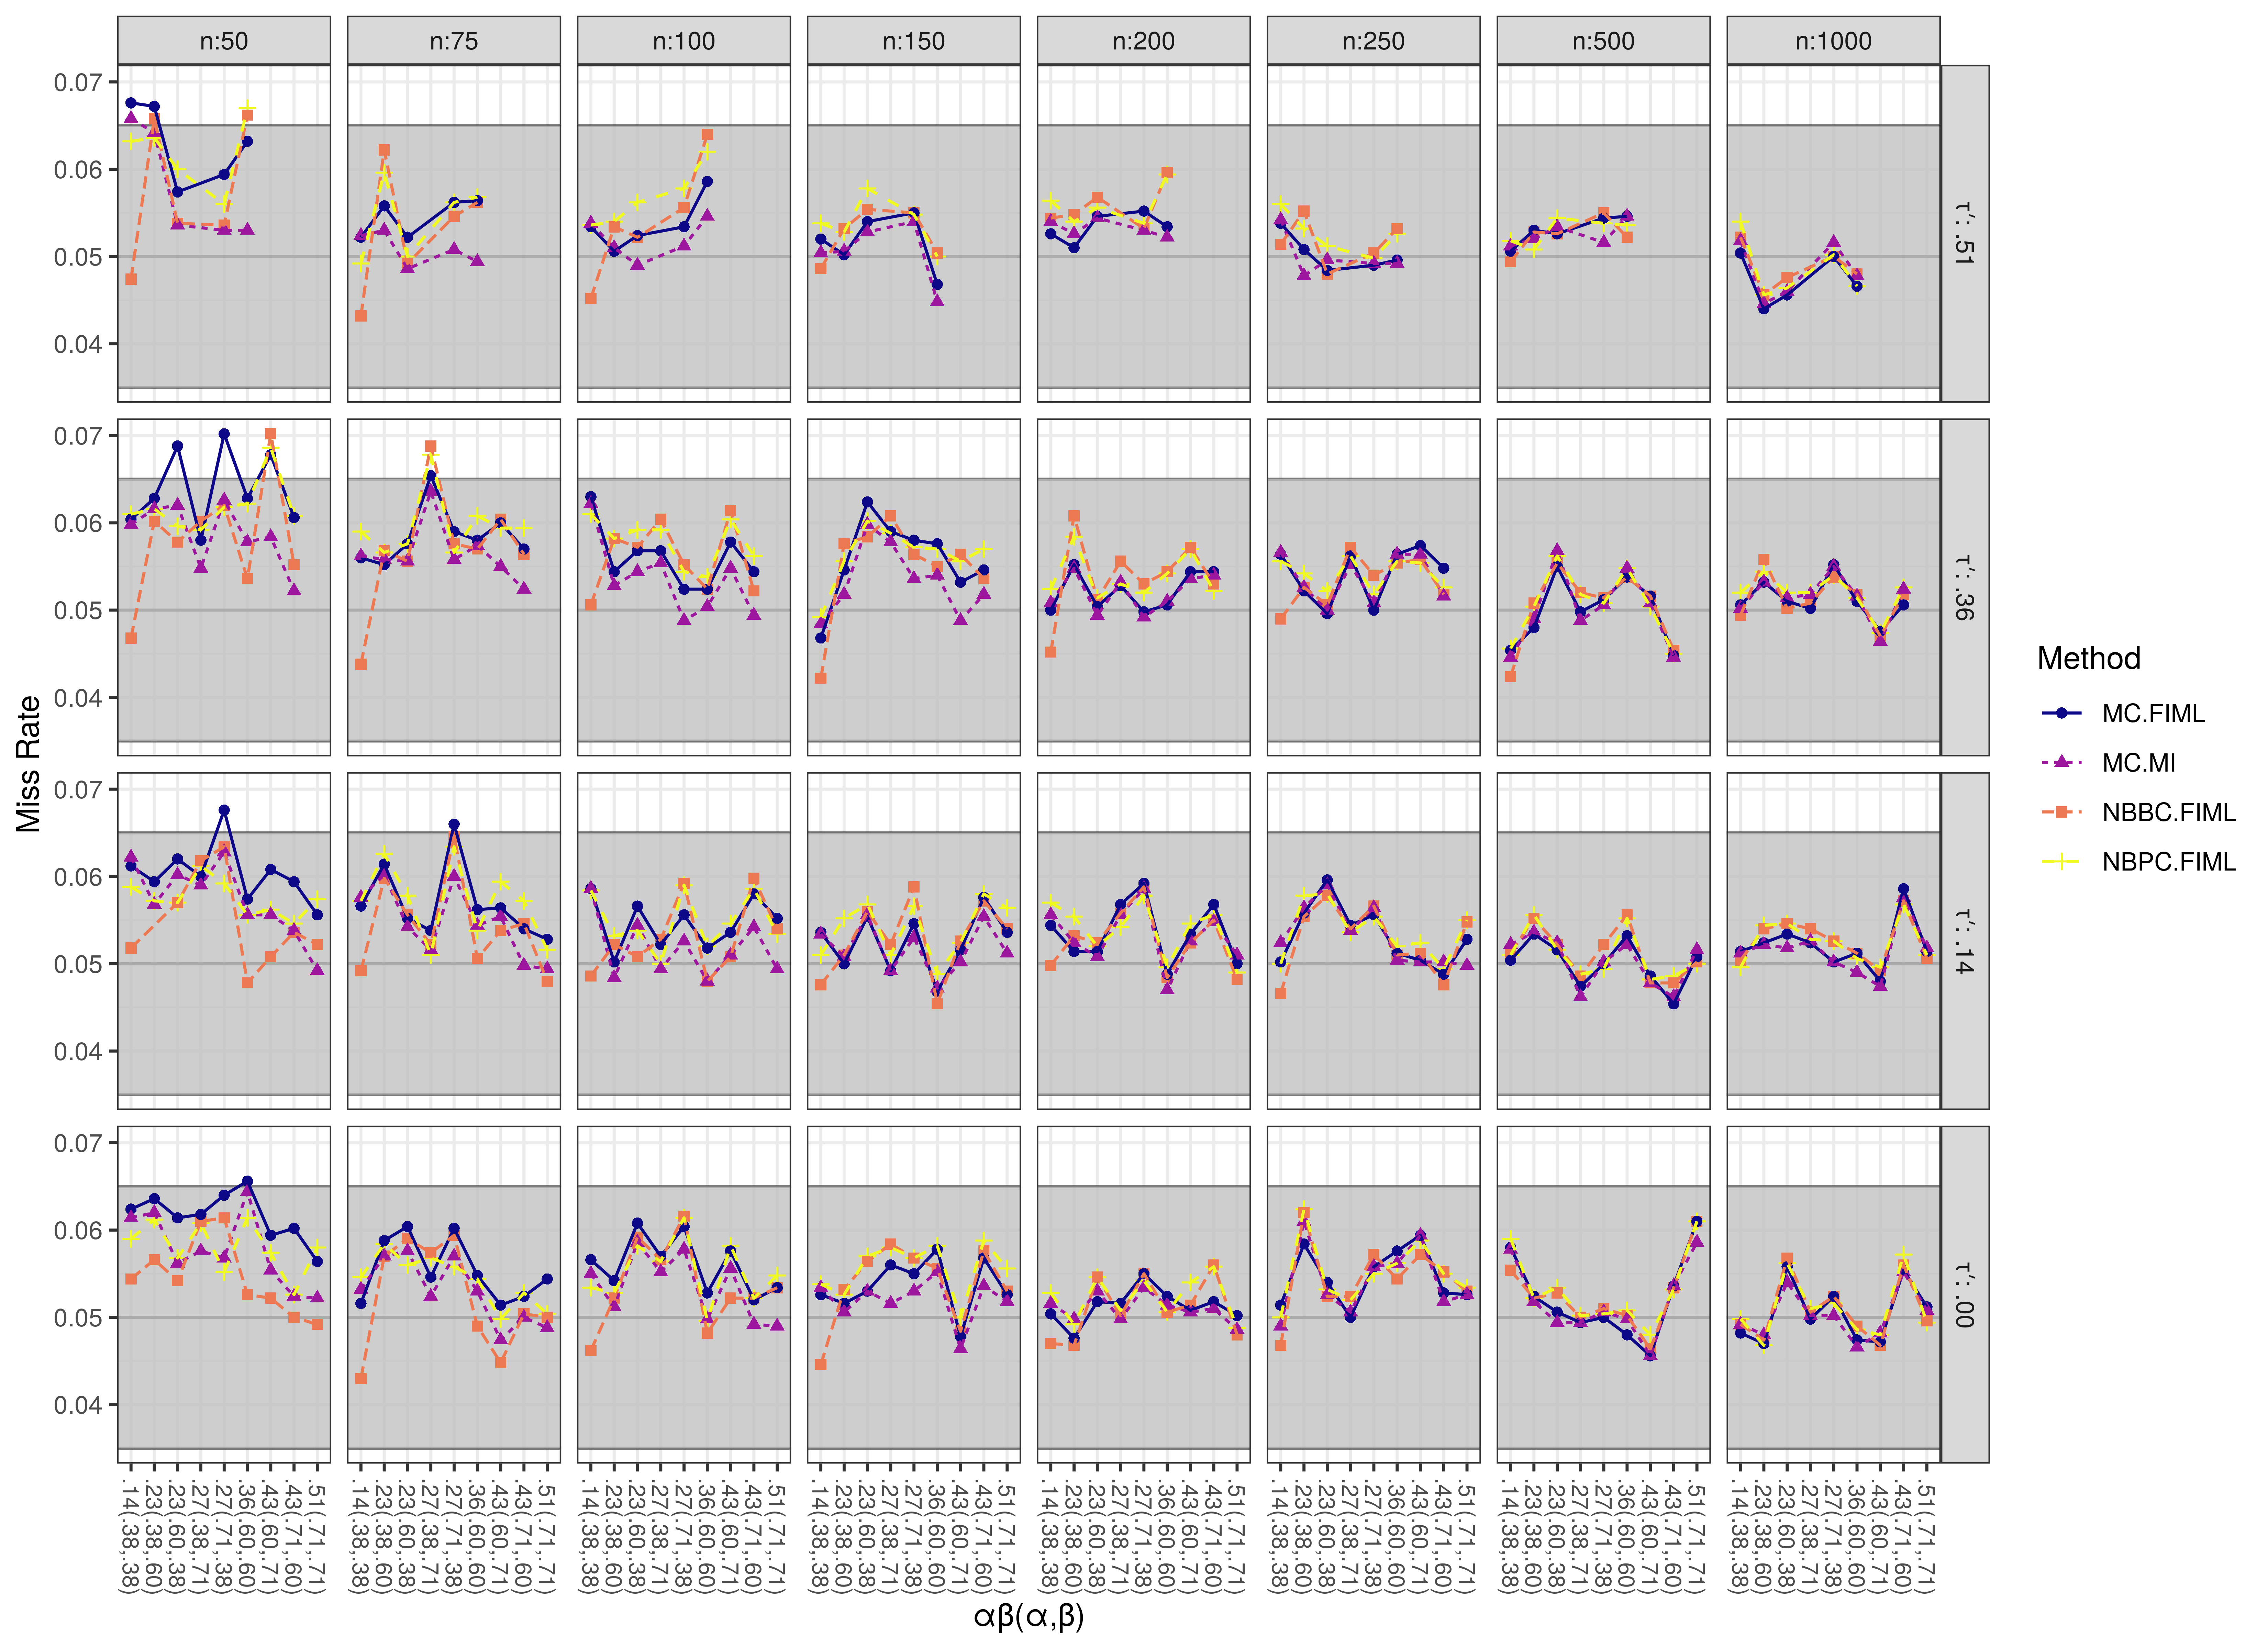
\includegraphics[scale=.60]{figures/png/mar-30-miss.png}
	\figurenote{
		${n}$ = sample size,
		${\alpha}$ = path from ${X}$ to ${M}$,
		${\beta}$ = path from ${M}$ to ${Y}$,
		${\tau}^{\prime}$ = direct effect,
		MC.FIML = Monte Carlo using FIML estimates,
		MC.MI = Monte Carlo using MI estimates,
		NBBC.FIML = Nonparametric bootstrap with bias-corrected confidence intervals using FIML,
        NBPC.FIML = Nonparametric bootstrap with percentile confidence intervals using FIML.
    }
	\label{fig:mar-30-miss}
\end{figure}

\newpage

\end{document}
